% ====================================================================================
\chapter{机器人运动学与动力学}
% ====================================================================================

\section*{让机器动起来}

\marginnote{Marc Raibert (1949--)是Boston Dynamics创始人。他让机器人第一次像动物一样奔跑、跳跃、翻跟头。他的秘诀？"先让它跳起来，再想怎么落地。"}

\vspace{0.5cm}
\noindent\textit{你的手臂有7个自由度，但你从来不需要"计算"如何拿起一杯咖啡。机器人却需要——它必须把"拿杯子"这个任务翻译成每个关节应该转多少度。}

试着做一个实验：伸出你的手，保持手掌位置不动，然后移动你的手肘。你会发现，即使手掌固定，手肘仍然可以在一个圆弧上运动。这说明什么？你的手臂有"多余"的自由度——完成"固定手掌"这个任务后，还剩下一些自由度可以用来做别的事情。

这个简单的观察背后，是机器人学中一个核心问题：\textbf{运动学}——关节角度和末端位置之间的关系。更深一层，当机器人需要推、拉、抓取物体时，我们还需要\textbf{动力学}——力、质量、加速度之间的关系。

本章将展示：第4章学到的拉格朗日力学如何直接应用于机器人。你会发现，关节力矩、接触力都是拉格朗日乘子的工程化身。

\begin{quote}
\textbf{本章目标}：机器人是拉格朗日力学最直接的工程应用——关节力、接触力都是拉格朗日乘子。本章将建立从"任务描述"到"关节力矩"的完整链条。
\end{quote}

% ------------------------------------------------------------------------------------
\section{从人手臂到机械臂}

\subsection{为什么机器人需要"算"？}

人类拿起一杯咖啡，大脑只需要想"拿杯子"，手臂就自动完成了。我们从不需要计算"肩关节转23度，肘关节转45度，腕关节转-12度"。

但机器人不同。机器人的"大脑"（控制器）收到的命令是"把末端移动到坐标(0.5, 0.3, 0.2)"，它必须计算出每个电机应该转多少度。这个过程叫做\textbf{逆运动学}。

反过来，如果我们知道每个关节的角度，要算出末端在哪里，这叫做\textbf{正运动学}。正运动学相对简单——就是一连串的几何变换。逆运动学则困难得多——它可能有多个解，也可能无解。

\begin{figure}[h]
\centering
\begin{tikzpicture}[scale=1.0]
    % 左边：关节空间
    \begin{scope}[shift={(-4,0)}]
        \node[draw, rounded corners, fill=blue!10, minimum width=3cm, minimum height=2cm] (joint) at (0,0) {
            \begin{tabular}{c}
            \textbf{关节空间} \\
            $q = (q_1, q_2, \ldots, q_n)$ \\
            \small 每个关节转多少度？
            \end{tabular}
        };
    \end{scope}
    
    % 右边：任务空间
    \begin{scope}[shift={(4,0)}]
        \node[draw, rounded corners, fill=red!10, minimum width=3cm, minimum height=2cm] (task) at (0,0) {
            \begin{tabular}{c}
            \textbf{任务空间} \\
            $x = (\text{位置, 姿态})$ \\
            \small 末端在哪里？朝哪？
            \end{tabular}
        };
    \end{scope}
    
    % 箭头
    \draw[->, thick, blue] (joint.east) -- (task.west) 
        node[midway, above] {正运动学 $x = f(q)$}
        node[midway, below] {\small 简单、唯一};
    \draw[->, thick, red, transform canvas={yshift=-1.5cm}] (task.west) -- (joint.east) 
        node[midway, above] {逆运动学 $q = f^{-1}(x)$}
        node[midway, below] {\small 困难、可能多解};
\end{tikzpicture}
\caption{机器人的两种"语言"：关节空间与任务空间}
\end{figure}

\subsection{自由度的概念}

\textbf{自由度}（Degrees of Freedom, DoF）是描述系统需要多少个独立参数才能完全确定其位置。

\begin{example}[日常生活中的自由度]
\begin{itemize}
    \item \textbf{门}：1个自由度（只能绕铰链转动）
    \item \textbf{抽屉}：1个自由度（只能前后滑动）
    \item \textbf{办公椅}：5-6个自由度（上下、前后、旋转、靠背倾斜...）
    \item \textbf{人的手臂}：7个自由度（肩3个 + 肘1个 + 腕3个）
    \item \textbf{人的手指}：每根手指约4个自由度
\end{itemize}
\end{example}

\marginnote{为什么人的手臂是7个自由度而不是6个？因为我们需要在固定手掌位置的同时，还能调整手肘位置（比如绕开障碍物）。这个"多出来"的自由度叫做\textbf{冗余自由度}。}

任务空间通常是6维的：3个位置 $(x, y, z)$ + 3个姿态（如欧拉角或四元数的3个独立分量）。

\begin{center}
\renewcommand{\arraystretch}{1.3}
\begin{tabular}{l|c|c|l}
\toprule
\textbf{机械臂类型} & \textbf{关节数 $n$} & \textbf{与任务空间比较} & \textbf{特点} \\
\midrule
SCARA（平面装配） & 4 & $n < 6$ & 只能在平面内运动 \\
典型工业臂 & 6 & $n = 6$ & 恰好完成6D任务 \\
人形机械臂 & 7 & $n > 6$ & 冗余，更灵活 \\
双臂机器人 & 14 & $n \gg 6$ & 高度冗余 \\
\bottomrule
\end{tabular}
\end{center}

% ------------------------------------------------------------------------------------
\section{运动学基础}

\subsection{齐次变换：旋转与平移的统一表示}

描述物体在三维空间中的位置和姿态，需要同时处理旋转和平移。\textbf{齐次变换矩阵}把这两者统一成一个 $4 \times 4$ 矩阵：

\marginnote{\textbf{D-H参数}：机器人运动学的标准表示法由Jacques Denavit和Richard Hartenberg于1955年提出。这套参数用4个数描述每个关节，使得任何串联机械臂都能用统一的框架分析。几乎所有工业机器人的技术手册都使用D-H参数。}

\begin{definition}[齐次变换]
\begin{equation}
T = \begin{bmatrix} R & p \\ 0 & 1 \end{bmatrix} \in SE(3)
\end{equation}
其中 $R \in SO(3)$ 是 $3 \times 3$ 旋转矩阵，$p \in \mathbb{R}^3$ 是平移向量。
\end{definition}

齐次变换的美妙之处在于：\textbf{多次变换可以通过矩阵乘法串联}。

\begin{example}[两次变换的串联]
假设坐标系A相对于世界坐标系的变换是 $T_A$，坐标系B相对于A的变换是 $T_B$，那么B相对于世界坐标系的变换是：
\[
T_{world \to B} = T_A \cdot T_B
\]
就这么简单！矩阵乘法帮我们处理了所有复杂的几何关系。
\end{example}

\subsection{正运动学：从关节到末端}

对于 $n$ 关节的机械臂，每个关节 $i$ 贡献一个变换 $T_i(q_i)$（取决于关节角 $q_i$）。末端相对于基座的变换是所有关节变换的乘积：

\begin{equation}
T_{end}(q) = T_1(q_1) \cdot T_2(q_2) \cdots T_n(q_n)
\end{equation}

\begin{example}[平面双连杆机械臂的正运动学]
考虑最简单的情况：两个连杆在平面内运动，长度分别为 $L_1$ 和 $L_2$。

\begin{figure}[h]
\centering
\begin{tikzpicture}[scale=1.5]
    % 坐标系
    \draw[->] (-0.5,0) -- (3,0) node[right] {$x$};
    \draw[->] (0,-0.5) -- (0,2) node[above] {$y$};
    
    % 连杆1
    \draw[very thick, blue] (0,0) -- ({1.5*cos(50)},{1.5*sin(50)});
    \node[blue, above left] at ({0.75*cos(50)},{0.75*sin(50)}) {$L_1$};
    
    % 连杆2
    \draw[very thick, red] ({1.5*cos(50)},{1.5*sin(50)}) -- 
        ({1.5*cos(50)+1.2*cos(50-30)},{1.5*sin(50)+1.2*sin(50-30)});
    \node[red, above right] at ({1.5*cos(50)+0.6*cos(50-30)},{1.5*sin(50)+0.6*sin(50-30)}) {$L_2$};
    
    % 关节
    \fill (0,0) circle (2pt);
    \fill ({1.5*cos(50)},{1.5*sin(50)}) circle (2pt);
    \fill ({1.5*cos(50)+1.2*cos(50-30)},{1.5*sin(50)+1.2*sin(50-30)}) circle (3pt);
    \node[right] at ({1.5*cos(50)+1.2*cos(50-30)},{1.5*sin(50)+1.2*sin(50-30)}) {末端 $(x,y)$};
    
    % 角度
    \draw[->] (0.5,0) arc (0:50:0.5);
    \node at (0.7,0.3) {$q_1$};
    
    \draw[->] ({1.5*cos(50)+0.4*cos(50)},{1.5*sin(50)+0.4*sin(50)}) 
        arc (50:20:0.4);
    \node at ({1.5*cos(50)+0.5},{1.5*sin(50)+0.1}) {$q_2$};
\end{tikzpicture}
\caption{平面双连杆机械臂}
\end{figure}

正运动学方程：
\begin{align}
x &= L_1 \cos q_1 + L_2 \cos(q_1 + q_2) \\
y &= L_1 \sin q_1 + L_2 \sin(q_1 + q_2)
\end{align}

这个公式很直观：
\begin{itemize}
    \item 第一项 $(L_1 \cos q_1, L_1 \sin q_1)$ 是肘关节的位置
    \item 第二项是从肘关节到末端的位移（方向是 $q_1 + q_2$）
\end{itemize}
\end{example}

\begin{example}[手算练习]
设 $L_1 = L_2 = 1$，$q_1 = 60°$，$q_2 = -30°$，求末端位置。

\textbf{解}：
\begin{align}
x &= \cos 60° + \cos(60° - 30°) = 0.5 + \cos 30° = 0.5 + 0.866 = 1.366 \\
y &= \sin 60° + \sin 30° = 0.866 + 0.5 = 1.366
\end{align}

末端位置约为 $(1.37, 1.37)$。
\end{example}

% ------------------------------------------------------------------------------------
\section{雅可比矩阵：连接速度与力的桥梁}

\subsection{为什么需要雅可比？}

正运动学告诉我们"位置"的关系：$x = f(q)$。但在控制中，我们经常需要知道"速度"的关系：关节转得多快，末端就移动得多快？

这就是\textbf{雅可比矩阵}的作用——它是 $f(q)$ 的一阶导数，描述速度的映射关系。

\begin{definition}[雅可比矩阵]
末端速度与关节速度的关系：
\begin{equation}
\dot{x} = J(q) \dot{q}
\end{equation}
其中 $J(q) = \frac{\partial f}{\partial q}$ 是 $m \times n$ 的雅可比矩阵（$m$是任务空间维度，$n$是关节数）。
\end{definition}

\begin{example}[双连杆机械臂的雅可比]
对正运动学方程求导：
\begin{equation}
J = \begin{bmatrix} 
\frac{\partial x}{\partial q_1} & \frac{\partial x}{\partial q_2} \\[6pt]
\frac{\partial y}{\partial q_1} & \frac{\partial y}{\partial q_2}
\end{bmatrix}
= \begin{bmatrix}
-L_1 \sin q_1 - L_2 \sin(q_1+q_2) & -L_2 \sin(q_1+q_2) \\
L_1 \cos q_1 + L_2 \cos(q_1+q_2) & L_2 \cos(q_1+q_2)
\end{bmatrix}
\end{equation}

注意 $J$ 依赖于当前位形 $q$——机械臂在不同姿态下，速度传递关系是不同的。
\end{example}

\subsection{力的对偶关系：雅可比的转置}

雅可比矩阵有一个神奇的性质：它的\textbf{转置}把末端力映射到关节力矩。

\begin{keytheorem}[title=力/力矩转换]
\begin{equation}
\boxed{\tau = J(q)^\top F}
\end{equation}
末端力 $F \in \mathbb{R}^m$ 需要关节力矩 $\tau \in \mathbb{R}^n$ 来平衡。
\end{keytheorem}

\begin{physicalmeaning}
这个公式来自\textbf{虚功原理}——关节空间做的虚功必须等于任务空间做的虚功：
\[
\delta W = \tau^\top \delta q = F^\top \delta x = F^\top J \delta q
\]
由于 $\delta q$ 是任意的，必有 $\tau = J^\top F$。

\textbf{直觉}：$J$ 把关节速度"放大"成末端速度，$J^\top$ 把末端力"缩小"成关节力矩。速度放大多少倍，力就缩小多少倍——这是杠杆原理的推广！
\end{physicalmeaning}

\begin{example}[力的传递]
双连杆机械臂，$L_1 = L_2 = 1$m，$q_1 = 90°$，$q_2 = 0°$（手臂竖直向上伸直）。

末端受到水平向右的力 $F = (10, 0)^\top$ N，求所需的关节力矩。

\textbf{解}：首先计算雅可比：
\[
J = \begin{bmatrix}
-\sin 90° - \sin 90° & -\sin 90° \\
\cos 90° + \cos 90° & \cos 90°
\end{bmatrix}
= \begin{bmatrix}
-2 & -1 \\
0 & 0
\end{bmatrix}
\]

然后：
\[
\tau = J^\top F = \begin{bmatrix} -2 & 0 \\ -1 & 0 \end{bmatrix} \begin{bmatrix} 10 \\ 0 \end{bmatrix}
= \begin{bmatrix} -20 \\ -10 \end{bmatrix} \text{ Nm}
\]

\textbf{物理解释}：要抵抗水平向右的力，两个关节都需要产生"逆时针"的力矩。肩关节力矩是肘关节的两倍，因为它到末端的力臂更长。
\end{example}

\subsection{奇异性：机械臂的"盲区"}

当雅可比矩阵不满秩时（$\det(J) = 0$ 对于方阵，或 $\text{rank}(J) < \min(m,n)$），机械臂处于\textbf{奇异位形}。

\begin{figure}[h]
\centering
\begin{tikzpicture}[scale=1.0]
    % 正常位形
    \begin{scope}[shift={(0,0)}]
        \draw[very thick, blue] (0,0) -- (1.5,1.2);
        \draw[very thick, red] (1.5,1.2) -- (3,0.3);
        \fill (0,0) circle (3pt);
        \fill (1.5,1.2) circle (3pt);
        \fill (3,0.3) circle (3pt);
        
        % 可达方向
        \draw[->, thick, green!60!black] (3,0.3) -- (3.7,0.8);
        \draw[->, thick, green!60!black] (3,0.3) -- (3.7,-0.2);
        \draw[->, thick, green!60!black] (3,0.3) -- (2.3,0.8);
        \node at (3.9,0.3) {\small 全方向可达};
        
        \node[below] at (1.5,-0.3) {\small 正常位形};
    \end{scope}
    
    % 奇异位形
    \begin{scope}[shift={(6,0)}]
        \draw[very thick, blue] (0,0) -- (1.5,0);
        \draw[very thick, red] (1.5,0) -- (3,0);
        \fill (0,0) circle (3pt);
        \fill (1.5,0) circle (3pt);
        \fill (3,0) circle (3pt);
        
        % 可达方向
        \draw[->, thick, green!60!black] (3,0) -- (3,0.7);
        \draw[->, thick, green!60!black] (3,0) -- (3,-0.7);
        \node[above] at (3,0.8) {\small 只能上下};
        
        % 不可达
        \draw[dashed, red] (3,0) -- (3.7,0);
        \node[red, right] at (3.7,0) {\small 无法移动};
        
        \node[below] at (1.5,-0.3) {\small 奇异位形（伸直）};
    \end{scope}
\end{tikzpicture}
\caption{奇异位形：手臂完全伸直时，末端无法沿手臂方向移动}
\end{figure}

奇异性带来两个问题：
\begin{enumerate}
    \item \textbf{速度不可达}：某些方向的末端速度无法通过任何关节速度实现
    \item \textbf{力放大}：在奇异方向上，即使很小的末端力也需要无穷大的关节力矩
\end{enumerate}

\begin{example}[伸直位形的奇异性]
当 $q_2 = 0$（手臂伸直）时：
\[
\det(J) = L_1 L_2 \sin q_2 = 0
\]

此时，两个连杆在一条直线上，末端无法沿这条直线方向移动——两个关节的转动都只能让末端垂直于手臂运动。

\textbf{生活类比}：当你的手臂完全伸直时，很难通过弯曲/伸展来让指尖向前移动。你必须先把手肘弯曲一点，才能向前够东西。
\end{example}

% ------------------------------------------------------------------------------------
\section{逆运动学：约束优化的工程应用}

\subsection{问题的本质}

逆运动学的问题是：给定目标末端位置 $x_d$，求关节角 $q$。

这是一个\textbf{方程求解问题}：
\[
f(q) = x_d
\]

但它经常被转化为\textbf{优化问题}——寻找"最好"的解：

\begin{keyformula}[title=逆运动学的优化形式]
\begin{equation}
\min_q \frac{1}{2}\|q - q_0\|^2 \quad \st \quad f(q) = x_d
\end{equation}

含义：在所有能到达目标的关节角中，选择离当前位置 $q_0$ 最近的。
\end{keyformula}

\begin{physicalmeaning}
为什么要用优化形式？
\begin{enumerate}
    \item 当 $n > m$（冗余机械臂）时，有无穷多解，需要选择标准
    \item 当 $n = m$ 时，可能有多个解（如手肘朝上或朝下），需要选择最自然的
    \item 可以方便地加入其他约束（关节限位、避障等）
\end{enumerate}
\end{physicalmeaning}

\subsection{拉格朗日方法求解}

构造拉格朗日函数：
\begin{equation}
\mathcal{L}(q, \lambda) = \frac{1}{2}\|q - q_0\|^2 + \lambda^\top (f(q) - x_d)
\end{equation}

KKT条件：
\begin{align}
\nabla_q \mathcal{L} &= (q - q_0) + J(q)^\top \lambda = 0 \\
\nabla_\lambda \mathcal{L} &= f(q) - x_d = 0
\end{align}

从第一式解出：
\begin{equation}
q = q_0 - J^\top \lambda
\end{equation}

\begin{physicalmeaning}
$\lambda$ 的物理意义是\textbf{约束力}：如果用一根刚性杆把末端固定在目标位置 $x_d$，需要在末端施加多大的力？

这个力通过 $J^\top$ 传递到关节空间，导致关节偏离"自然位置" $q_0$。
\end{physicalmeaning}

\subsection{牛顿迭代法求解逆运动学}

逆运动学方程 $f(q) = x_d$ 是非线性的，没有通用的解析解。我们需要用数值方法。

\paragraph{核心思想：线性化}

回想微积分中的泰勒展开：对于一元函数 $f(x)$，在 $x_0$ 附近：
\[
f(x) \approx f(x_0) + f'(x_0)(x - x_0)
\]

对于向量函数 $f(q)$，类似地：
\[
f(q) \approx f(q_0) + J(q_0)(q - q_0)
\]

其中 $J = \frac{\partial f}{\partial q}$ 就是雅可比矩阵——它是导数在多元情况下的推广。

\paragraph{迭代算法}

既然我们想让 $f(q) = x_d$，把上面的近似代入：
\[
x_d \approx f(q_0) + J(q_0)(q - q_0)
\]

整理得：
\[
q \approx q_0 + J(q_0)^{-1}(x_d - f(q_0))
\]

这给出了一个迭代公式：

\begin{enumerate}
    \item 从初始猜测 $q^{(0)}$ 开始（比如当前关节角度）
    \item 计算当前末端位置：$x^{(k)} = f(q^{(k)})$
    \item 计算误差：$e = x_d - x^{(k)}$（"还差多远"）
    \item 计算雅可比：$J = J(q^{(k)})$
    \item 求解线性方程：$J \cdot \Delta q = e$（"关节要怎么动"）
    \item 更新关节角：$q^{(k+1)} = q^{(k)} + \Delta q$
    \item 如果 $\|e\|$ 足够小，停止；否则回到第2步
\end{enumerate}

\begin{figure}[h]
\centering
\begin{tikzpicture}[scale=1.2]
    % 工作空间
    \draw[->] (0,0) -- (4,0) node[right] {$x$};
    \draw[->] (0,0) -- (0,3) node[above] {$y$};
    
    % 目标点
    \fill[red] (3,2) circle (3pt) node[right] {目标 $x_d$};
    
    % 迭代轨迹
    \fill[blue] (1,0.5) circle (2pt) node[below] {$x^{(0)}$};
    \fill[blue] (1.8,1.2) circle (2pt) node[below left] {$x^{(1)}$};
    \fill[blue] (2.5,1.7) circle (2pt) node[below left] {$x^{(2)}$};
    \fill[blue] (2.9,1.95) circle (2pt);
    
    \draw[->, blue, thick] (1,0.5) -- (1.75,1.15);
    \draw[->, blue, thick] (1.8,1.2) -- (2.45,1.65);
    \draw[->, blue, thick] (2.5,1.7) -- (2.85,1.92);
    
    % 说明
    \node at (2,-0.5) {\small 末端位置逐步逼近目标};
\end{tikzpicture}
\caption{牛顿迭代法：每一步都让末端更接近目标}
\end{figure}

\begin{example}[牛顿迭代的手算演示]
双连杆机械臂，$L_1 = L_2 = 1$，目标位置 $x_d = (1.2, 0.9)$。

从初始猜测 $q^{(0)} = (30°, 30°) = (0.524, 0.524)$ rad 开始。

\textbf{第一次迭代}：

1. 计算当前末端位置：
\begin{align}
x^{(0)} &= \cos(30°) + \cos(60°) = 0.866 + 0.5 = 1.366 \\
y^{(0)} &= \sin(30°) + \sin(60°) = 0.5 + 0.866 = 1.366
\end{align}

2. 计算误差：
\[
e = x_d - x^{(0)} = (1.2, 0.9) - (1.366, 1.366) = (-0.166, -0.466)
\]

3. 计算雅可比（代入 $q_1 = 30°$，$q_2 = 30°$）：
\[
J = \begin{bmatrix}
-\sin 30° - \sin 60° & -\sin 60° \\
\cos 30° + \cos 60° & \cos 60°
\end{bmatrix}
= \begin{bmatrix}
-1.366 & -0.866 \\
1.366 & 0.5
\end{bmatrix}
\]

4. 求解 $J \Delta q = e$：
\[
\Delta q = J^{-1} e \approx (-0.05, -0.35) \text{ rad} = (-2.9°, -20.1°)
\]

5. 更新：
\[
q^{(1)} = q^{(0)} + \Delta q = (27.1°, 9.9°)
\]

继续迭代几次后，会收敛到精确解。

\textbf{关键观察}：每次迭代都在解一个\textbf{线性}方程组 $J \Delta q = e$。非线性问题被分解成了一系列线性问题！
\end{example}

\paragraph{当雅可比不可逆时怎么办？}

如果 $n \neq m$（关节数不等于任务空间维度），或者机械臂处于奇异位形，$J$ 不可逆。这时用\textbf{伪逆}：

\[
\Delta q = J^\dagger e, \quad \text{其中 } J^\dagger = J^\top(JJ^\top)^{-1}
\]

伪逆给出的是\textbf{最小范数解}——在所有能消除误差的 $\Delta q$ 中，选择最小的那个。

\begin{example}[几何解法 vs 迭代解法]
双连杆机械臂，$L_1 = L_2 = 1$，目标位置 $(1.0, 1.0)$。

\textbf{几何解法}（利用特殊结构）：

由于连杆等长，可以用余弦定理直接求解。

设末端到原点的距离为 $r = \sqrt{1^2 + 1^2} = \sqrt{2}$。

\begin{figure}[h]
\centering
\begin{tikzpicture}[scale=1.5]
    % 坐标系
    \draw[->] (-0.3,0) -- (1.8,0) node[right] {$x$};
    \draw[->] (0,-0.3) -- (0,1.8) node[above] {$y$};
    
    % 两种解
    % 解1：手肘朝上
    \draw[very thick, blue] (0,0) -- (0,1) -- (1,1);
    \fill[blue] (0,1) circle (2pt) node[left] {\small 肘};
    
    % 解2：手肘朝下（虚线）
    \draw[thick, blue, dashed] (0,0) -- (1,0) -- (1,1);
    \fill[blue, opacity=0.5] (1,0) circle (2pt) node[below] {\small 肘};
    
    % 目标点
    \fill[red] (1,1) circle (3pt) node[above right] {$(1,1)$};
    
    % 原点
    \fill (0,0) circle (2pt) node[below left] {$O$};
    
    % 距离标注
    \draw[<->, gray] (0.1,0.1) -- (0.9,0.9);
    \node[gray] at (0.7,0.3) {$r=\sqrt{2}$};
\end{tikzpicture}
\caption{逆运动学的两个解：手肘朝上或朝下}
\end{figure}

在三角形中，由余弦定理：
\[
r^2 = L_1^2 + L_2^2 - 2L_1 L_2 \cos(\pi - q_2)
\]

注意 $\pi - q_2$ 是三角形的内角，而 $q_2$ 是肘关节的弯曲角度。

代入数值：
\[
2 = 1 + 1 + 2 \cdot 1 \cdot 1 \cdot \cos q_2 \quad \Rightarrow \quad \cos q_2 = 0 \quad \Rightarrow \quad q_2 = \pm 90°
\]

两个解：
\begin{itemize}
    \item $q_2 = +90°$：手肘朝上（图中实线）
    \item $q_2 = -90°$：手肘朝下（图中虚线）
\end{itemize}

取 $q_2 = 90°$，代入正运动学方程求 $q_1$：
\begin{align}
1 &= \cos q_1 + \cos(q_1 + 90°) = \cos q_1 - \sin q_1 \\
1 &= \sin q_1 + \sin(q_1 + 90°) = \sin q_1 + \cos q_1
\end{align}

两式相加：$2 = 2\cos q_1$，所以 $\cos q_1 = 1$，$q_1 = 0°$。

\textbf{验证}：
\[
x = \cos 0° + \cos 90° = 1 + 0 = 1 \quad \checkmark
\]
\[
y = \sin 0° + \sin 90° = 0 + 1 = 1 \quad \checkmark
\]

\textbf{总结}：几何解法快速直接，但只适用于简单结构。牛顿迭代法适用于任意复杂的机械臂。
\end{example}

\subsection{冗余机械臂与零空间}

\paragraph{什么是冗余？}

当机械臂的关节数 $n$ 大于任务空间维度 $m$ 时，我们说它是\textbf{冗余}的。

\begin{center}
\renewcommand{\arraystretch}{1.3}
\begin{tabular}{l|c|c|l}
\toprule
\textbf{例子} & \textbf{关节数 $n$} & \textbf{任务维度 $m$} & \textbf{冗余度 $n-m$} \\
\midrule
平面双连杆 & 2 & 2 & 0（恰好） \\
典型工业臂 & 6 & 6 & 0（恰好） \\
人的手臂 & 7 & 6 & 1 \\
双臂机器人 & 14 & 6（单手任务） & 8 \\
蛇形机器人 & 20+ & 6 & 14+ \\
\bottomrule
\end{tabular}
\end{center}

\paragraph{冗余意味着什么？}

冗余意味着逆运动学有\textbf{无穷多解}。直觉上：完成同一个任务，有很多种姿势可以选择。

\begin{example}[人手臂的冗余]
做一个实验：
\begin{enumerate}
    \item 把你的手掌放在桌面上，固定不动
    \item 保持手掌位置和朝向不变，移动你的手肘
\end{enumerate}

你会发现，手肘可以在一个弧线上移动，而手掌完全不动！这就是冗余带来的自由度。

这个"额外"的自由度让我们能够：
\begin{itemize}
    \item 绕开障碍物（比如在狭窄空间中工作）
    \item 避免撞到自己的身体
    \item 找到更舒适的姿势
\end{itemize}
\end{example}

\paragraph{零空间的数学描述}

\begin{definition}[零空间]
雅可比矩阵 $J$ 的\textbf{零空间}（Null Space）是所有满足 $J v = 0$ 的向量 $v$ 的集合：
\[
\mathcal{N}(J) = \{ v \in \mathbb{R}^n : Jv = 0 \}
\]
\end{definition}

\textbf{物理意义}：如果关节速度 $\dot{q}$ 在零空间中，那么 $\dot{x} = J\dot{q} = 0$——末端不动！

换句话说，零空间运动是"内部运动"——关节在动，但末端静止。

\begin{figure}[h]
\centering
\begin{tikzpicture}[scale=1.0]
    % 左图：三连杆机械臂，两种构型
    \begin{scope}[shift={(0,0)}]
        \node at (2,-2) {\textbf{(a) 三连杆机械臂}};
        
        % 构型1
        \draw[very thick, blue] (0,0) -- (1,1.5) -- (2.5,1.8) -- (3.5,1);
        \fill (0,0) circle (2pt);
        \fill (1,1.5) circle (2pt);
        \fill (2.5,1.8) circle (2pt);
        \fill[red] (3.5,1) circle (3pt);
        
        % 构型2（虚线）
        \draw[thick, blue, dashed] (0,0) -- (1.5,0.8) -- (2.8,1.5) -- (3.5,1);
        \fill[blue, opacity=0.3] (1.5,0.8) circle (2pt);
        \fill[blue, opacity=0.3] (2.8,1.5) circle (2pt);
        
        % 说明
        \node[red] at (3.5,0.5) {\small 末端固定};
        \draw[<->, dashed, gray] (1,1.5) .. controls (1.3,1.1) .. (1.5,0.8);
        \node[gray] at (0.5,1) {\scriptsize 零空间运动};
    \end{scope}
    
    % 右图：零空间示意
    \begin{scope}[shift={(7,0)}]
        \node at (2,-2) {\textbf{(b) 零空间示意}};
        
        % 关节空间
        \draw[->] (0,0) -- (3.5,0) node[right] {$\dot{q}_1$};
        \draw[->] (0,0) -- (0,2.5) node[above] {$\dot{q}_2$};
        
        % 零空间（一条线）
        \draw[very thick, green!60!black] (-0.5,-0.3) -- (3,1.8);
        \node[green!60!black] at (3.2,2) {$\mathcal{N}(J)$};
        
        % 一个向量
        \draw[->, thick, blue] (0,0) -- (2,1.2);
        \node[blue] at (1.5,0.5) {$\dot{q} \in \mathcal{N}(J)$};
        
        % 说明
        \node at (1.5,-0.8) {\small 沿此方向运动};
        \node at (1.5,-1.2) {\small 末端速度为零};
    \end{scope}
\end{tikzpicture}
\caption{零空间运动：关节在动，末端不动}
\end{figure}

\paragraph{冗余逆运动学的通解}

当 $n > m$ 时，逆运动学的解可以写成：

\begin{keyformula}[title=冗余逆运动学的通解]
\begin{equation}
\dot{q} = \underbrace{J^\dagger \dot{x}_d}_{\text{完成主任务}} + \underbrace{(I - J^\dagger J) z}_{\text{零空间运动}}
\end{equation}
其中：
\begin{itemize}
    \item $J^\dagger = J^\top(JJ^\top)^{-1}$ 是\textbf{伪逆}
    \item $\dot{x}_d$ 是期望的末端速度
    \item $z \in \mathbb{R}^n$ 是\textbf{任意向量}
    \item $(I - J^\dagger J)$ 是\textbf{零空间投影矩阵}
\end{itemize}
\end{keyformula}

\begin{physicalmeaning}
这个公式说的是：
\begin{enumerate}
    \item 第一项 $J^\dagger \dot{x}_d$ 保证末端以期望速度 $\dot{x}_d$ 运动
    \item 第二项 $(I - J^\dagger J) z$ 不影响末端（因为它在零空间中）
    \item $z$ 可以自由选择，用来实现\textbf{次级目标}
\end{enumerate}
\end{physicalmeaning}

\paragraph{次级目标的例子}

$z$ 可以怎么选？常见的选择：

\begin{enumerate}
    \item \textbf{远离关节限位}：
    \[
    z = k \nabla_q W(q), \quad W(q) = \sum_i \frac{1}{(q_i - q_i^{min})(q_i^{max} - q_i)}
    \]
    $W$ 在关节接近限位时变大，梯度方向指向"远离限位"。
    
    \item \textbf{避开障碍物}：
    \[
    z = k \nabla_q d(q)
    \]
    其中 $d(q)$ 是机械臂与障碍物的最近距离。
    
    \item \textbf{最小化能量}：
    \[
    z = -k \nabla_q \|\tau\|^2
    \]
    让关节力矩尽可能小。
\end{enumerate}

\begin{example}[冗余的实际应用]
想象一个7自由度机械臂在一个有障碍物的环境中工作：

\begin{figure}[h]
\centering
\begin{tikzpicture}[scale=0.9]
    % 障碍物
    \fill[gray!40] (2,0.5) rectangle (2.5,2);
    \node at (2.25,2.3) {\small 障碍物};
    
    % 构型1：会撞到障碍物
    \draw[thick, red, dashed] (0,0) -- (1,1) -- (2.2,1.2) -- (3.5,0.8);
    \fill[red, opacity=0.5] (2.2,1.2) circle (3pt);
    \node[red] at (1.5,1.5) {\small 碰撞！};
    
    % 构型2：绕开障碍物
    \draw[very thick, blue] (0,0) -- (0.8,1.5) -- (1.5,2.2) -- (3.5,0.8);
    \fill (0,0) circle (2pt);
    \fill (0.8,1.5) circle (2pt);
    \fill (1.5,2.2) circle (2pt) node[above] {\small 肘抬高};
    \fill[red] (3.5,0.8) circle (3pt) node[right] {\small 末端};
    
    % 说明
    \node at (1.75,-0.5) {\small 利用零空间绕开障碍物};
\end{tikzpicture}
\caption{冗余自由度让机械臂能够在保持末端位置的同时避开障碍物}
\end{figure}

两种构型的末端位置相同，但只有蓝色构型能避开障碍物。冗余自由度提供了这种灵活性。
\end{example}

% ------------------------------------------------------------------------------------
\section{机器人动力学：力与运动的关系}

\subsection{为什么需要动力学？}

到目前为止，我们讨论的运动学只关心\textbf{几何关系}——关节角度和末端位置的对应。但实际控制机器人时，我们需要知道：

\begin{quote}
\textit{电机应该输出多大的力矩，才能让机械臂按照期望的方式运动？}
\end{quote}

这就是\textbf{动力学}要回答的问题。

\begin{example}[直觉理解]
想象你在举哑铃：
\begin{itemize}
    \item 如果哑铃很重，你需要很大的力才能举起来（质量大）
    \item 如果你想举得很快，需要更大的力（加速度大）
    \item 即使哑铃静止不动，你也需要用力来抵抗重力
    \item 如果哑铃在转动，你会感到一些"奇怪"的力（科氏力、离心力）
\end{itemize}

机器人动力学就是要把这些直觉变成精确的数学公式。
\end{example}

\subsection{复习：拉格朗日方程}

在第4章，我们学过拉格朗日方程：
\begin{equation}
\frac{d}{dt}\frac{\partial L}{\partial \dot{q}_i} - \frac{\partial L}{\partial q_i} = Q_i
\end{equation}

其中：
\begin{itemize}
    \item $L = T - V$ 是拉格朗日量（动能减势能）
    \item $q_i$ 是广义坐标（对机器人来说就是关节角度）
    \item $Q_i$ 是广义力（对机器人来说就是关节力矩 $\tau_i$）
\end{itemize}

这个方程的美妙之处在于：只要写出动能和势能的表达式，力学方程就自动出来了！

\subsection{机器人的动能}

\paragraph{单连杆的动能}

考虑一根绕端点转动的杆（单摆），质量 $m$，长度 $L$，假设质量集中在末端：

\begin{figure}[h]
\centering
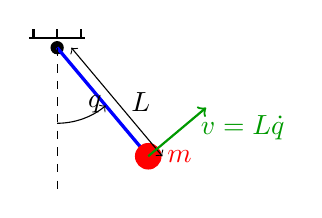
\begin{tikzpicture}[scale=1.2]
    % 固定点
    \fill (0,0) circle (2pt);
    \draw[thick] (-0.3,0.1) -- (0.3,0.1);
    \draw[thick] (-0.25,0.1) -- (-0.25,0.2);
    \draw[thick] (0,0.1) -- (0,0.2);
    \draw[thick] (0.25,0.1) -- (0.25,0.2);
    
    % 连杆
    \draw[very thick, blue] (0,0) -- ({1.5*sin(40)},{-1.5*cos(40)});
    
    % 质点
    \fill[red] ({1.5*sin(40)},{-1.5*cos(40)}) circle (4pt);
    \node[red, right] at ({1.5*sin(40)+0.1},{-1.5*cos(40)}) {$m$};
    
    % 角度
    \draw[dashed] (0,0) -- (0,-1.5);
    \draw[->] (0,-0.8) arc (-90:-50:0.8);
    \node at (0.4,-0.6) {$q$};
    
    % 长度
    \draw[<->] (0.15,0) -- ({1.5*sin(40)+0.15},{-1.5*cos(40)});
    \node[right] at ({0.75*sin(40)+0.2},{-0.75*cos(40)}) {$L$};
    
    % 速度
    \draw[->, thick, green!60!black] ({1.5*sin(40)},{-1.5*cos(40)}) -- 
        ({1.5*sin(40)+0.8*cos(40)},{-1.5*cos(40)+0.8*sin(40)});
    \node[green!60!black] at ({1.5*sin(40)+1},{-1.5*cos(40)+0.3}) {$v = L\dot{q}$};
\end{tikzpicture}
\caption{单摆：最简单的"机器人"}
\end{figure}

质点的速度大小为 $v = L\dot{q}$（圆周运动），所以动能是：
\begin{equation}
T = \frac{1}{2}mv^2 = \frac{1}{2}m(L\dot{q})^2 = \frac{1}{2}mL^2 \dot{q}^2
\end{equation}

我们可以定义\textbf{转动惯量} $I = mL^2$，则 $T = \frac{1}{2}I\dot{q}^2$。

\paragraph{多连杆的动能}

对于多连杆机械臂，每个连杆都在运动，总动能是各部分之和。关键观察是：每个连杆的速度取决于\textbf{所有它之前的关节}的角度和角速度。

最终，总动能可以写成：
\begin{equation}
T = \frac{1}{2} \dot{q}^\top M(q) \dot{q}
\end{equation}

其中 $M(q)$ 是 $n \times n$ 的\textbf{质量矩阵}（也叫惯性矩阵）。

\begin{physicalmeaning}
$M(q)$ 的物理意义：
\begin{itemize}
    \item $M_{ii}$：第 $i$ 个关节单独转动时的"有效惯量"
    \item $M_{ij}$（$i \neq j$）：关节 $i$ 和 $j$ 之间的"惯性耦合"
    \item $M$ 依赖于位形 $q$：机械臂伸直时和弯曲时，惯量不同！
\end{itemize}
\end{physicalmeaning}

\begin{example}[伸直 vs 弯曲的惯量]
想象一根双连杆机械臂：

\begin{figure}[h]
\centering
\begin{tikzpicture}[scale=1.0]
    % 伸直
    \begin{scope}[shift={(0,0)}]
        \draw[very thick, blue] (0,0) -- (2,0) -- (4,0);
        \fill (0,0) circle (2pt);
        \fill (2,0) circle (2pt);
        \fill[red] (4,0) circle (3pt);
        \draw[->] (0,-0.5) arc (-90:0:0.5);
        \node at (0.7,-0.3) {$\dot{q}_1$};
        \node at (2,-1) {\small 伸直：转动惯量大};
    \end{scope}
    
    % 弯曲
    \begin{scope}[shift={(6,0)}]
        \draw[very thick, blue] (0,0) -- (1.5,0) -- (1.5,-1.5);
        \fill (0,0) circle (2pt);
        \fill (1.5,0) circle (2pt);
        \fill[red] (1.5,-1.5) circle (3pt);
        \draw[->] (0,-0.5) arc (-90:0:0.5);
        \node at (0.7,-0.3) {$\dot{q}_1$};
        \node at (1,-2) {\small 弯曲：转动惯量小};
    \end{scope}
\end{tikzpicture}
\caption{质量矩阵依赖于位形}
\end{figure}

当手臂伸直时，末端离肩关节很远，绕肩关节转动时需要更大的力矩。这体现在 $M_{11}$ 更大。

当手臂弯曲时，末端离肩关节近，转动惯量变小。
\end{example}

\subsection{机器人的势能}

对于大多数机器人，势能只来自重力：
\begin{equation}
V = \sum_i m_i g h_i(q)
\end{equation}

其中 $h_i(q)$ 是第 $i$ 个连杆质心的高度（取决于关节角度 $q$）。

\subsection{推导动力学方程}

现在让我们用拉格朗日方程推导机器人的动力学。

\paragraph{第一步：计算 $\frac{\partial L}{\partial \dot{q}}$}

\begin{align}
\frac{\partial L}{\partial \dot{q}} &= \frac{\partial T}{\partial \dot{q}} - \frac{\partial V}{\partial \dot{q}} \\
&= \frac{\partial}{\partial \dot{q}} \left( \frac{1}{2} \dot{q}^\top M(q) \dot{q} \right) - 0 \\
&= M(q) \dot{q}
\end{align}

（这里用到了 $\frac{\partial}{\partial x}(x^\top A x) = 2Ax$ 对于对称矩阵 $A$。）

\paragraph{第二步：计算 $\frac{d}{dt}\frac{\partial L}{\partial \dot{q}}$}

\begin{align}
\frac{d}{dt}(M(q)\dot{q}) &= \dot{M}(q)\dot{q} + M(q)\ddot{q}
\end{align}

这里 $\dot{M}$ 是 $M$ 对时间的导数，它依赖于 $\dot{q}$。

\paragraph{第三步：计算 $\frac{\partial L}{\partial q}$}

\begin{align}
\frac{\partial L}{\partial q} &= \frac{\partial T}{\partial q} - \frac{\partial V}{\partial q}
\end{align}

$\frac{\partial T}{\partial q}$ 来自 $M(q)$ 对 $q$ 的依赖，$\frac{\partial V}{\partial q}$ 是重力产生的力。

\paragraph{第四步：整理}

把所有项放在一起，经过仔细整理（具体推导需要一些技巧），最终得到：

\begin{keyformula}[title=机器人动力学标准形式]
\begin{equation}
\boxed{M(q)\ddot{q} + C(q, \dot{q})\dot{q} + G(q) = \tau}
\end{equation}
\end{keyformula}

\begin{center}
\renewcommand{\arraystretch}{1.5}
\begin{tabular}{c|l|p{7cm}}
\toprule
\textbf{符号} & \textbf{名称} & \textbf{物理意义} \\
\midrule
$M(q)\ddot{q}$ & 惯性项 & 加速关节需要的力矩，就像 $F = ma$ \\
$C(q, \dot{q})\dot{q}$ & 科氏力/离心力 & 速度引起的"假想力"，旋转坐标系中才有 \\
$G(q)$ & 重力项 & 抵抗重力需要的力矩 \\
$\tau$ & 关节力矩 & 电机需要输出的力矩 \\
\bottomrule
\end{tabular}
\end{center}

\begin{example}[单摆的完整推导]
让我们对单摆完整做一遍拉格朗日推导。

\textbf{设置}：质量 $m$，长度 $L$，关节角 $q$（从竖直向下测量）。

\textbf{动能}：
\[
T = \frac{1}{2}mL^2\dot{q}^2
\]

\textbf{势能}（以铰链为零势能点）：
\[
V = -mgL\cos q
\]

注意：当 $q = 0$（竖直向下）时，$V = -mgL$（最低）；当 $q = 90°$（水平）时，$V = 0$。

\textbf{拉格朗日量}：
\[
L = T - V = \frac{1}{2}mL^2\dot{q}^2 + mgL\cos q
\]

\textbf{计算各项}：
\begin{align}
\frac{\partial L}{\partial \dot{q}} &= mL^2\dot{q} \\
\frac{d}{dt}\frac{\partial L}{\partial \dot{q}} &= mL^2\ddot{q} \\
\frac{\partial L}{\partial q} &= -mgL\sin q
\end{align}

\textbf{拉格朗日方程}：
\[
mL^2\ddot{q} - (-mgL\sin q) = \tau
\]

即：
\[
\boxed{mL^2\ddot{q} + mgL\sin q = \tau}
\]

\textbf{对比标准形式}：
\begin{itemize}
    \item $M = mL^2$（常数，因为单摆只有一个关节）
    \item $C = 0$（单关节没有科氏力）
    \item $G = mgL\sin q$（重力产生的力矩）
\end{itemize}

\textbf{物理检验}：
\begin{itemize}
    \item 当 $q = 0$（竖直向下）：$G = 0$，不需要力矩来维持
    \item 当 $q = 90°$（水平）：$G = mgL$，需要最大力矩
    \item 当 $q = 180°$（竖直向上）：$G = 0$，但这是不稳定平衡
\end{itemize}
\end{example}

\begin{example}[双连杆机械臂的动力学（概念性）]
对于双连杆机械臂，动力学方程会更复杂。质量矩阵是 $2 \times 2$：

\[
M(q) = \begin{bmatrix}
M_{11}(q_2) & M_{12}(q_2) \\
M_{12}(q_2) & M_{22}
\end{bmatrix}
\]

注意：
\begin{itemize}
    \item $M_{11}$ 依赖于 $q_2$（肘关节角度）：手臂弯曲时，肩关节的有效惯量变小
    \item $M_{22}$ 是常数：肘关节的惯量不受其他关节影响
    \item $M_{12} = M_{21}$：对称性来自动能的二次型性质
\end{itemize}

科氏力矩阵 $C$ 包含 $\dot{q}_1^2$ 和 $\dot{q}_1\dot{q}_2$ 等项——这些是快速运动时产生的"假想力"。

重力向量 $G$ 包含 $\sin$ 和 $\cos$ 项——取决于各连杆的角度。

具体表达式很长，通常用符号计算软件导出。
\end{example}

\subsection{动力学的重要性质}

机器人动力学有几个重要的数学性质，它们对控制设计很有用：

\paragraph{性质1：质量矩阵对称正定}
\[
M(q) = M(q)^\top, \quad M(q) > 0
\]

\textbf{物理意义}：动能 $T = \frac{1}{2}\dot{q}^\top M \dot{q}$ 总是正的（只要有运动）。

\paragraph{性质2：$\dot{M} - 2C$ 反对称}
\[
\dot{q}^\top (\dot{M} - 2C) \dot{q} = 0
\]

\textbf{物理意义}：这保证了能量守恒。如果没有外力（$\tau = 0$）且忽略重力，系统能量 $T$ 保持不变。

\begin{proof}[简单说明]
对动能求时间导数：
\begin{align}
\frac{dT}{dt} &= \frac{d}{dt}\left(\frac{1}{2}\dot{q}^\top M \dot{q}\right) \\
&= \frac{1}{2}\dot{q}^\top \dot{M} \dot{q} + \dot{q}^\top M \ddot{q}
\end{align}

把 $M\ddot{q} = \tau - C\dot{q} - G$ 代入：
\begin{align}
\frac{dT}{dt} &= \frac{1}{2}\dot{q}^\top \dot{M} \dot{q} + \dot{q}^\top (\tau - C\dot{q} - G) \\
&= \dot{q}^\top \tau - \dot{q}^\top G + \frac{1}{2}\dot{q}^\top (\dot{M} - 2C) \dot{q}
\end{align}

如果 $\dot{M} - 2C$ 反对称，最后一项为零，于是：
\[
\frac{dT}{dt} = \dot{q}^\top \tau - \dot{q}^\top G = \text{功率输入} - \text{重力功率}
\]

这正是能量守恒的表达！
\end{proof}

\paragraph{性质3：线性于参数}

动力学方程可以写成：
\[
M(q)\ddot{q} + C(q,\dot{q})\dot{q} + G(q) = Y(q, \dot{q}, \ddot{q}) \theta
\]

其中 $Y$ 是已知的矩阵（只依赖于运动状态），$\theta$ 是物理参数向量（质量、惯量、质心位置等）。

\textbf{应用}：这个性质让我们能够通过测量运动和力矩来\textbf{辨识}机器人的物理参数。

% ------------------------------------------------------------------------------------
\section{接触力学：当机器人碰到东西时}

\subsection{为什么接触很重要？}

机器人与世界交互几乎总是通过接触：
\begin{itemize}
    \item 机械臂抓取物体
    \item 腿式机器人行走
    \item 工业机器人装配零件
    \item 手术机器人操作组织
\end{itemize}

没有接触力的分析，我们无法理解机器人如何真正"做事"。

\begin{example}[行走的秘密]
当你走路时，脚蹬地，地面给你一个向前的摩擦力，推动你前进。

如果地面是完美光滑的（没有摩擦），你只能原地踏步——就像在冰面上一样。

机器人行走也是如此：地面反作用力是推动机器人前进的"动力来源"。
\end{example}

\subsection{接触力如何进入动力学方程}

当机器人与环境接触时，接触点受到\textbf{接触力} $\lambda_c$。这个力如何影响关节运动？

答案是通过\textbf{雅可比转置}——和末端力传递完全一样！

\begin{keyformula}[title=带接触的动力学方程]
\begin{equation}
M(q)\ddot{q} + C(q,\dot{q})\dot{q} + G(q) = \tau + J_c(q)^\top \lambda_c
\end{equation}

其中：
\begin{itemize}
    \item $J_c(q)$ 是接触点的雅可比矩阵
    \item $\lambda_c$ 是接触力（在接触点处）
    \item $J_c^\top \lambda_c$ 是接触力产生的\textbf{广义力}（在关节空间）
\end{itemize}
\end{keyformula}

\begin{physicalmeaning}
$J_c^\top$ 把接触点的力"传递"到关节空间，就像 $J^\top$ 把末端力传递到关节一样。

这正是我们在约束优化中见过的\textbf{拉格朗日乘子}！$\lambda_c$ 是接触约束的乘子，它自动给出了维持约束所需的力。
\end{physicalmeaning}

\subsection{接触力的物理约束}

接触力不是任意的，它必须满足物理约束：

\paragraph{约束1：不能穿透}

设 $\phi(q)$ 是接触间隙（机器人与环境之间的最近距离）：
\begin{itemize}
    \item $\phi > 0$：没有接触
    \item $\phi = 0$：正在接触
    \item $\phi < 0$：穿透（物理上不允许！）
\end{itemize}

约束：$\phi(q) \geq 0$

\paragraph{约束2：法向力是推力}

接触面只能"推"不能"拉"（除非有吸盘）：
\[
\lambda_n \geq 0
\]

其中 $\lambda_n$ 是法向接触力。

\paragraph{约束3：互补松弛}

这是最关键的条件：
\[
\lambda_n \cdot \phi(q) = 0
\]

\textbf{含义}：
\begin{itemize}
    \item 如果 $\phi > 0$（不接触），则 $\lambda_n = 0$（没有力）
    \item 如果 $\lambda_n > 0$（有力），则 $\phi = 0$（必须接触）
\end{itemize}

\begin{figure}[h]
\centering
\begin{tikzpicture}[scale=1.4]
    % 地面
    \fill[gray!20] (-0.5,-0.1) rectangle (8,0);
    \draw[thick] (-0.5,0) -- (8,0);
    
    % 状态1：悬空
    \begin{scope}[shift={(1,0)}]
        \draw[thick, blue, fill=blue!20] (0,1) circle (0.4);
        \node at (0,1) {\small 球};
        \draw[->, red, thick] (0,0.6) -- (0,0.15) node[right] {$mg$};
        
        \node at (0,-0.4) {\small $\phi > 0$};
        \node at (0,-0.7) {\small $\lambda = 0$};
        \node at (0,1.7) {\small \textbf{悬空}};
    \end{scope}
    
    % 状态2：静止接触
    \begin{scope}[shift={(3.5,0)}]
        \draw[thick, blue, fill=blue!20] (0,0.4) circle (0.4);
        \node at (0,0.4) {\small 球};
        \draw[->, red, thick] (0,0.4) -- (0,-0.25) node[right] {$mg$};
        \draw[->, green!60!black, thick] (0,0) -- (0,0.65) node[left] {$\lambda$};
        
        \node at (0,-0.4) {\small $\phi = 0$};
        \node at (0,-0.7) {\small $\lambda = mg$};
        \node at (0,1.1) {\small \textbf{静止接触}};
    \end{scope}
    
    % 状态3：滑动接触
    \begin{scope}[shift={(6,0)}]
        \draw[thick, blue, fill=blue!20] (0,0.4) circle (0.4);
        \node at (0,0.4) {\small 球};
        \draw[->, red, thick] (0,0.4) -- (0,-0.25);
        \draw[->, green!60!black, thick] (0,0) -- (0,0.65);
        \draw[->, orange, thick] (0,0) -- (0.5,0) node[above] {$f$};
        \draw[->, blue, thick] (0.4,0.4) -- (0.9,0.4) node[above] {$v$};
        
        \node at (0,-0.4) {\small $\phi = 0$};
        \node at (0,-0.7) {\small $|f| = \mu\lambda$};
        \node at (0,1.1) {\small \textbf{滑动接触}};
    \end{scope}
\end{tikzpicture}
\caption{接触的三种状态}
\end{figure}

\begin{insightbox}
互补松弛条件 $\lambda \cdot \phi = 0$ 和线性规划中的互补松弛完全一样！

在线性规划中："免费的资源没人用，稀缺的资源才有价格"。

在接触力学中："悬空时没有力，接触时才有力"。

这是同一个数学结构在不同领域的体现。
\end{insightbox}

\subsection{摩擦力与库仑锥}

除了法向力，接触通常还有\textbf{摩擦力}（切向力）。

\paragraph{库仑摩擦模型}

最常用的摩擦模型是库仑模型：
\begin{itemize}
    \item 静摩擦：当物体静止时，摩擦力可以是任意方向，但大小受限
    \item 动摩擦：当物体滑动时，摩擦力与速度方向相反，大小正比于法向力
\end{itemize}

数学表达：
\[
\|f_t\| \leq \mu \lambda_n
\]

其中 $f_t$ 是切向力，$\mu$ 是摩擦系数，$\lambda_n$ 是法向力。

\paragraph{摩擦锥}

这个不等式定义了一个\textbf{锥形区域}：接触力必须在锥内。

\begin{figure}[h]
\centering
\begin{tikzpicture}[scale=1.2]
    % 三维摩擦锥
    \begin{scope}[shift={(0,0)}]
        % 底面（椭圆表示圆）
        \draw[thick, gray, dashed] (0,0) ellipse (1.5 and 0.5);
        
        % 锥面
        \draw[thick, green!60!black, fill=green!10, opacity=0.5] 
            (0,0) -- (-1.5,0) -- (0,2.5) -- cycle;
        \draw[thick, green!60!black, fill=green!10, opacity=0.5] 
            (0,0) -- (1.5,0) -- (0,2.5) -- cycle;
        \draw[thick, green!60!black] (0,0) -- (0,2.5);
        
        % 顶点
        \fill (0,0) circle (2pt);
        
        % 一个可行的力
        \draw[->, very thick, blue] (0,0) -- (0.5,1.8);
        \node[blue, right] at (0.5,1.8) {$\lambda$（可行）};
        
        % 一个不可行的力
        \draw[->, very thick, red, dashed] (0,0) -- (1.8,0.8);
        \node[red, right] at (1.8,0.8) {（滑动）};
        
        % 标注
        \node at (0,-1.2) {\small 法向：$\lambda_n$};
        \draw[<->] (-1.7,0) -- (-1.7,2.5) node[midway, left] {\small $\lambda_n$};
        \draw[<->] (-1.5,-0.7) -- (1.5,-0.7) node[midway, below] {\small $\mu\lambda_n$};
    \end{scope}
    
    % 二维示意
    \begin{scope}[shift={(5,0)}]
        % 地面
        \fill[gray!20] (-1.5,-0.1) rectangle (1.5,0);
        \draw[thick] (-1.5,0) -- (1.5,0);
        
        % 摩擦锥（二维）
        \fill[green!20, opacity=0.5] (0,0) -- (-1,2) -- (1,2) -- cycle;
        \draw[thick, green!60!black] (0,0) -- (-1,2);
        \draw[thick, green!60!black] (0,0) -- (1,2);
        
        % 角度标注
        \draw[dashed] (0,0) -- (0,2);
        \draw (0,0.8) arc (90:117:0.8);
        \node at (-0.4,1) {\small $\theta$};
        \node at (1.3,1.5) {\small $\tan\theta = \mu$};
        
        % 说明
        \node at (0,-0.8) {\small 二维摩擦锥};
    \end{scope}
\end{tikzpicture}
\caption{摩擦锥：接触力必须在锥内才能保持静止}
\end{figure}

\paragraph{摩擦锥与优化}

摩擦锥约束 $\|f_t\| \leq \mu \lambda_n$ 是一个\textbf{二阶锥约束}（Second-Order Cone Constraint）。

带摩擦的接触问题可以formulate为\textbf{二阶锥规划}（SOCP），这是凸优化的一种，可以高效求解。

\begin{example}[机器人抓取]
当机械臂抓取一个物体时，手指与物体之间的接触力必须满足：
\begin{enumerate}
    \item 法向力为正（推而不拉）
    \item 摩擦力在锥内（不滑动）
    \item 合力平衡物体重力
\end{enumerate}

这是一个带锥约束的力平衡问题，可以用凸优化求解最优抓取力。

\begin{figure}[h]
\centering
\begin{tikzpicture}[scale=1.0]
    % 物体
    \fill[blue!20] (0,0) rectangle (2,1.5);
    \draw[thick] (0,0) rectangle (2,1.5);
    \node at (1,0.75) {物体};
    
    % 左手指
    \fill[gray!40] (-0.5,0.4) rectangle (0,1.1);
    \draw[thick] (-0.5,0.4) rectangle (0,1.1);
    
    % 右手指
    \fill[gray!40] (2,0.4) rectangle (2.5,1.1);
    \draw[thick] (2,0.4) rectangle (2.5,1.1);
    
    % 接触力
    \draw[->, thick, green!60!black] (0,0.75) -- (0.7,0.75) node[above] {$\lambda_1$};
    \draw[->, thick, green!60!black] (2,0.75) -- (1.3,0.75) node[above] {$\lambda_2$};
    
    % 重力
    \draw[->, thick, red] (1,0) -- (1,-0.7) node[right] {$mg$};
    
    % 摩擦锥示意
    \draw[dashed, green!60!black] (0,0.75) -- (0.4,1.1);
    \draw[dashed, green!60!black] (0,0.75) -- (0.4,0.4);
    \draw[dashed, green!60!black] (2,0.75) -- (1.6,1.1);
    \draw[dashed, green!60!black] (2,0.75) -- (1.6,0.4);
\end{tikzpicture}
\caption{抓取中的接触力必须在摩擦锥内}
\end{figure}
\end{example}

\subsection{接触问题的数学结构}

把所有约束放在一起，接触动力学可以写成一个\textbf{互补问题}（Complementarity Problem）：

\begin{keyformula}[title=接触动力学的数学形式]
\begin{align}
M(q)\ddot{q} + C\dot{q} + G &= \tau + J_c^\top \lambda_c \quad \text{（动力学）} \\
\phi(q) &\geq 0 \quad \text{（不穿透）} \\
\lambda_n &\geq 0 \quad \text{（推力）} \\
\lambda_n \cdot \phi &= 0 \quad \text{（互补松弛）} \\
\|f_t\| &\leq \mu \lambda_n \quad \text{（摩擦锥）}
\end{align}
\end{keyformula}

这个问题是\textbf{非光滑}的（因为互补条件在接触/分离瞬间不可微），数值求解需要特殊的算法。

现代机器人仿真器（如 MuJoCo、Drake、PyBullet）都实现了高效的接触求解器。

% ------------------------------------------------------------------------------------
\section{综合案例：双连杆机械臂的完整分析}

让我们把本章的所有内容整合起来，完整分析一个双连杆机械臂。

\subsection{问题描述}

\begin{figure}[h]
\centering
\begin{tikzpicture}[scale=1.5]
    % 坐标系
    \draw[->] (-0.5,0) -- (3,0) node[right] {$x$};
    \draw[->] (0,-0.5) -- (0,2.5) node[above] {$y$};
    
    % 连杆1
    \draw[very thick, blue] (0,0) -- ({1.5*cos(50)},{1.5*sin(50)});
    \fill[blue!30] ({0.75*cos(50)},{0.75*sin(50)}) circle (3pt);
    \node[blue] at ({0.75*cos(50)-0.3},{0.75*sin(50)}) {$m_1$};
    
    % 连杆2
    \draw[very thick, red] ({1.5*cos(50)},{1.5*sin(50)}) -- 
        ({1.5*cos(50)+1.2*cos(20)},{1.5*sin(50)+1.2*sin(20)});
    \fill[red!30] ({1.5*cos(50)+0.6*cos(20)},{1.5*sin(50)+0.6*sin(20)}) circle (3pt);
    \node[red] at ({1.5*cos(50)+0.6*cos(20)+0.3},{1.5*sin(50)+0.6*sin(20)}) {$m_2$};
    
    % 关节
    \fill (0,0) circle (2pt) node[below left] {$O$};
    \fill ({1.5*cos(50)},{1.5*sin(50)}) circle (2pt);
    \fill[green!60!black] ({1.5*cos(50)+1.2*cos(20)},{1.5*sin(50)+1.2*sin(20)}) circle (3pt);
    \node[green!60!black, right] at ({1.5*cos(50)+1.2*cos(20)},{1.5*sin(50)+1.2*sin(20)}) {末端};
    
    % 角度
    \draw[->] (0.6,0) arc (0:50:0.6);
    \node at (0.9,0.35) {$q_1$};
    
    \draw[->] ({1.5*cos(50)+0.4*cos(50)},{1.5*sin(50)+0.4*sin(50)}) arc (50:20:0.4);
    \node at ({1.5*cos(50)+0.55},{1.5*sin(50)+0.1}) {$q_2$};
    
    % 长度标注
    \draw[<->, gray] (0.1,-0.1) -- ({1.5*cos(50)+0.1},{1.5*sin(50)-0.1});
    \node[gray] at (0.5,0.7) {$L_1$};
    
    \draw[<->, gray] ({1.5*cos(50)+0.1},{1.5*sin(50)+0.1}) -- 
        ({1.5*cos(50)+1.2*cos(20)+0.1},{1.5*sin(50)+1.2*sin(20)+0.1});
    \node[gray] at ({1.5*cos(50)+0.8},{1.5*sin(50)+0.5}) {$L_2$};
\end{tikzpicture}
\caption{双连杆机械臂示意图}
\end{figure}

\textbf{参数}：
\begin{itemize}
    \item 连杆长度：$L_1 = L_2 = 1$ m
    \item 连杆质量：$m_1 = 2$ kg，$m_2 = 1$ kg（集中在连杆末端）
    \item 重力加速度：$g = 9.8$ m/s²
\end{itemize}

\subsection{运动学分析}

\paragraph{正运动学}

末端位置：
\begin{align}
x &= L_1 \cos q_1 + L_2 \cos(q_1 + q_2) \\
y &= L_1 \sin q_1 + L_2 \sin(q_1 + q_2)
\end{align}

\paragraph{雅可比矩阵}

\begin{equation}
J = \begin{bmatrix}
-L_1 \sin q_1 - L_2 \sin(q_1+q_2) & -L_2 \sin(q_1+q_2) \\
L_1 \cos q_1 + L_2 \cos(q_1+q_2) & L_2 \cos(q_1+q_2)
\end{bmatrix}
\end{equation}

\paragraph{奇异性分析}

行列式：
\[
\det(J) = L_1 L_2 [\cos q_1 \sin(q_1+q_2) - \sin q_1 \cos(q_1+q_2)] = L_1 L_2 \sin q_2
\]

奇异位形：$q_2 = 0$ 或 $q_2 = \pi$（手臂伸直或完全折叠）

\subsection{逆运动学计算}

\textbf{任务}：将末端移动到 $(0.8, 1.0)$。

\paragraph{Step 1：检查可达性}

末端到原点的距离：$r = \sqrt{0.8^2 + 1.0^2} = 1.28$ m

可达范围：$|L_1 - L_2| \leq r \leq L_1 + L_2$，即 $0 \leq r \leq 2$

$r = 1.28$ 在范围内，目标可达。

\paragraph{Step 2：求解 $q_2$}

由余弦定理（或直接展开正运动学方程）：
\[
x^2 + y^2 = L_1^2 + L_2^2 + 2L_1 L_2 \cos q_2
\]

代入：
\[
1.64 = 1 + 1 + 2 \cos q_2 \quad \Rightarrow \quad \cos q_2 = -0.18
\]

$q_2 = \pm 100.4°$

取 $q_2 = 100.4°$（手肘朝上）。

\paragraph{Step 3：求解 $q_1$}

设 $\alpha = \arctan(y/x) = \arctan(1.0/0.8) = 51.3°$

设 $\beta = \arctan\left(\frac{L_2 \sin q_2}{L_1 + L_2 \cos q_2}\right) = \arctan\left(\frac{0.985}{0.82}\right) = 50.2°$

则 $q_1 = \alpha - \beta = 1.1°$（手肘朝上的解）

或 $q_1 = \alpha + \beta = 101.5°$（手肘朝下的解）

\textbf{验证}（取 $q_1 = 1.1°$，$q_2 = 100.4°$）：
\begin{align}
x &= \cos 1.1° + \cos 101.5° = 1.0 - 0.2 = 0.8 \quad \checkmark \\
y &= \sin 1.1° + \sin 101.5° = 0.02 + 0.98 = 1.0 \quad \checkmark
\end{align}

\subsection{静力学分析}

\textbf{问题}：要保持机械臂在位置 $(q_1, q_2) = (1.1°, 100.4°)$ 静止，需要多大的关节力矩？

在静止状态，动力学方程简化为：
\[
G(q) = \tau
\]

重力项：
\begin{align}
G_1 &= m_1 g \frac{L_1}{2} \cos q_1 + m_2 g (L_1 \cos q_1 + \frac{L_2}{2} \cos(q_1+q_2)) \\
G_2 &= m_2 g \frac{L_2}{2} \cos(q_1+q_2)
\end{align}

（这里假设质量均匀分布在连杆上，所以用 $L/2$。如果质量集中在末端，用 $L$。）

代入数值：
\begin{align}
G_1 &= 2 \times 9.8 \times 0.5 \times \cos 1.1° + 1 \times 9.8 \times (1 \times \cos 1.1° + 0.5 \times \cos 101.5°) \\
&= 9.8 + 9.8 \times (1 - 0.1) = 9.8 + 8.8 = 18.6 \text{ Nm}
\end{align}

\begin{align}
G_2 &= 1 \times 9.8 \times 0.5 \times \cos 101.5° = -1.0 \text{ Nm}
\end{align}

\textbf{解读}：
\begin{itemize}
    \item 肩关节需要 $\tau_1 = 18.6$ Nm 的正力矩（逆时针）来抵抗重力
    \item 肘关节需要 $\tau_2 = -1.0$ Nm 的负力矩（顺时针）
\end{itemize}

\subsection{末端力分析}

\textbf{问题}：如果末端受到水平向右的力 $F = (10, 0)$ N，需要额外多大的关节力矩？

由 $\tau = J^\top F$：

先计算当前位形的雅可比：
\[
J = \begin{bmatrix}
-\sin 1.1° - \sin 101.5° & -\sin 101.5° \\
\cos 1.1° + \cos 101.5° & \cos 101.5°
\end{bmatrix}
= \begin{bmatrix}
-1.0 & -0.98 \\
0.8 & -0.2
\end{bmatrix}
\]

然后：
\[
\tau = J^\top F = \begin{bmatrix} -1.0 & 0.8 \\ -0.98 & -0.2 \end{bmatrix} \begin{bmatrix} 10 \\ 0 \end{bmatrix}
= \begin{bmatrix} -10 \\ -9.8 \end{bmatrix} \text{ Nm}
\]

\textbf{解读}：要抵抗水平向右的力，两个关节都需要产生负（顺时针）力矩。

\subsection{总结}

这个案例展示了本章主要概念的应用：
\begin{enumerate}
    \item 正运动学：$q \to x$
    \item 雅可比矩阵：速度和力的传递
    \item 逆运动学：$x \to q$（可能有多解）
    \item 奇异性：某些位形下运动受限
    \item 静力学：重力平衡
    \item 力传递：$\tau = J^\top F$
\end{enumerate}

% ------------------------------------------------------------------------------------
% 代码演示结果
\begin{figure}[htbp]
\centering
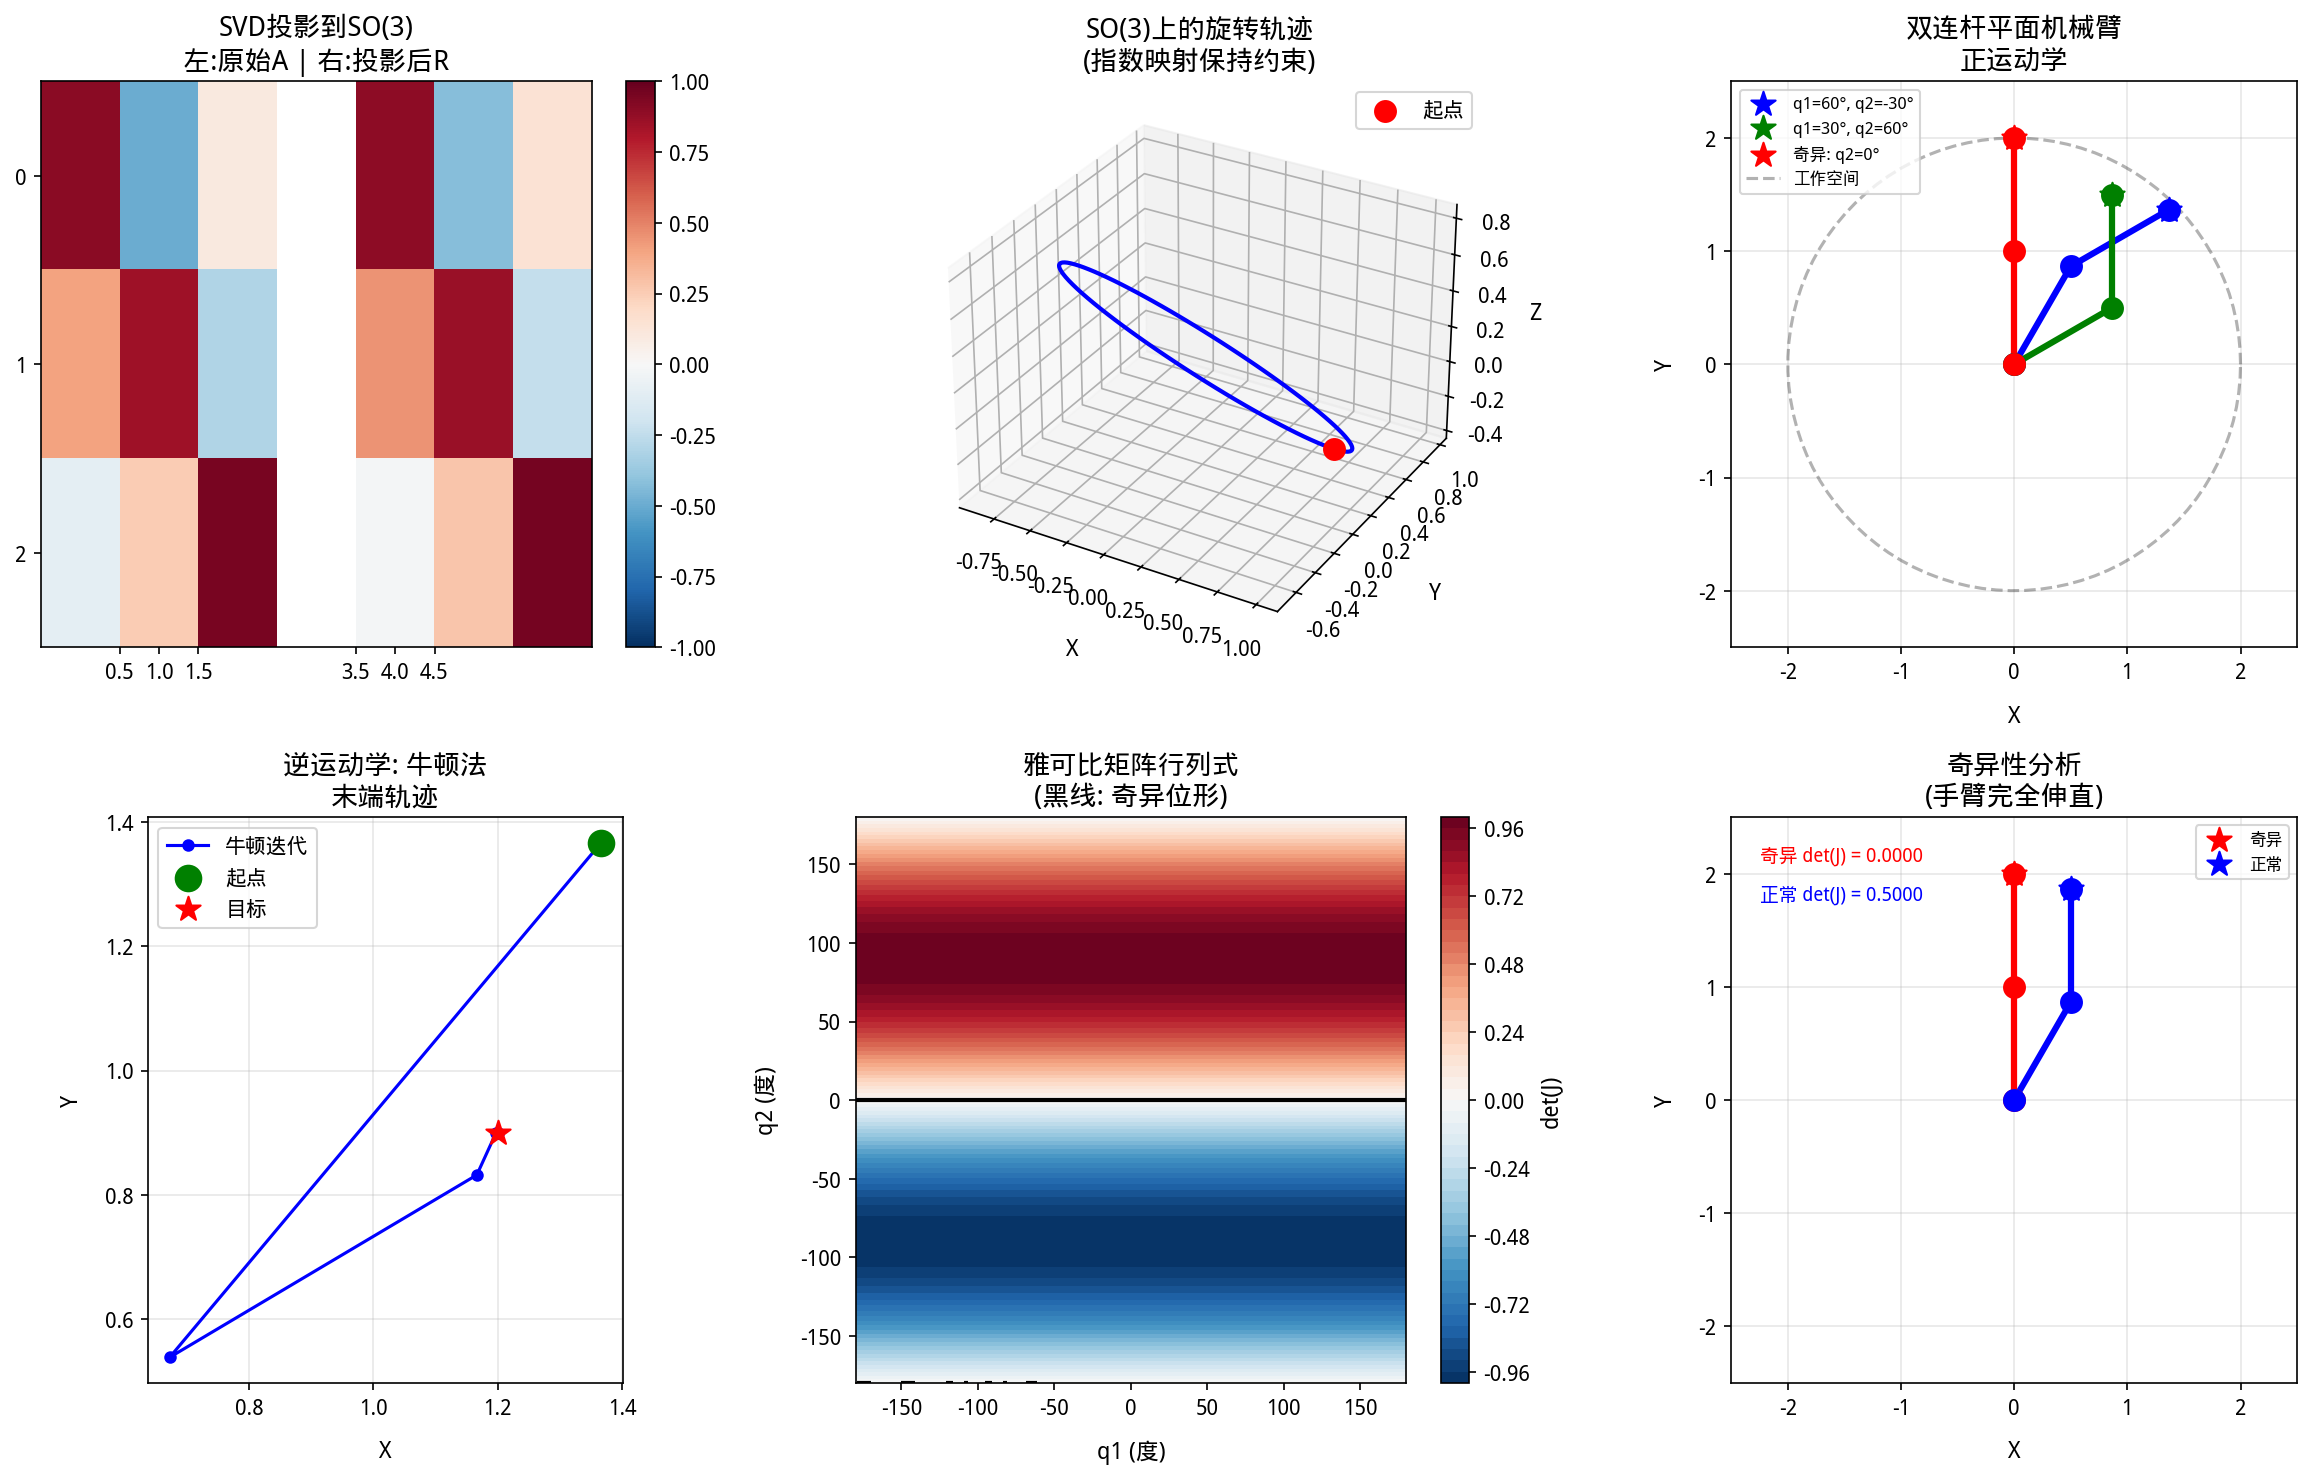
\includegraphics[width=0.98\textwidth]{figs/chap07_fig1.png}
\caption{机器人运动学与动力学演示。（1）SVD投影到SO(3)：将任意矩阵投影为有效旋转矩阵；（2）指数映射演示：在SO(3)流形上的正确旋转更新轨迹；（3）双连杆机械臂正运动学与工作空间；（4）牛顿法求解逆运动学的迭代收敛过程；（5）雅可比行列式热图，黑线标示奇异位形（$q_2 = 0, \pm\pi$）；（6）奇异性分析：手臂完全伸直时的奇异位形对比正常位形。代码验证：力传递结果$\tau = (-20, -10)$ Nm与书中一致。}
\label{fig:chap07_robotics}
\end{figure}

% ------------------------------------------------------------------------------------
\section{本章小结}

\begin{enumerate}
    \item \textbf{运动学}描述位置关系：正运动学 $x = f(q)$ 简单且唯一，逆运动学 $q = f^{-1}(x)$ 复杂且可能多解。
    
    \item \textbf{雅可比矩阵}是核心工具：$J$ 映射速度（$\dot{x} = J\dot{q}$），$J^\top$ 映射力（$\tau = J^\top F$）。这来自虚功原理。
    
    \item \textbf{奇异性}限制了机械臂的能力：在奇异位形，某些方向无法运动，某些方向力矩发散。
    
    \item \textbf{冗余}提供了额外自由度：零空间运动不影响末端，可用于次级目标（避障、远离限位等）。
    
    \item \textbf{动力学}来自拉格朗日方程：$M\ddot{q} + C\dot{q} + G = \tau$，把关节力矩与运动联系起来。
    
    \item \textbf{接触力}是拉格朗日乘子：互补条件 $\lambda \phi = 0$ 描述"接触才有力"，与线性规划的对偶理论一脉相承。
\end{enumerate}

\begin{unification}[title=$\lambda$ 在机器人学中的多重身份]
\begin{center}
\renewcommand{\arraystretch}{1.4}
\begin{tabular}{l|l|l}
\toprule
\textbf{场景} & \textbf{$\lambda$ 的含义} & \textbf{与优化的联系} \\
\midrule
逆运动学 & 末端约束力 & 等式约束的乘子 \\
关节限位 & 限位反力 & 不等式约束的乘子 \\
接触力 & 地面反作用力 & 互补约束的乘子 \\
闭链机构 & 环路内力 & 代数约束的乘子 \\
\bottomrule
\end{tabular}
\end{center}
\end{unification}

\begin{insightbox}
机器人学是约束优化最直接的工程应用。每一个关节限位、每一次接触、每一个任务目标，都对应着一个约束，而拉格朗日乘子 $\lambda$ 就是这些约束的"代言人"——它把抽象的几何限制转化为具体的物理力。

当你看到一个机械臂优雅地抓取物体，或者一个机器人稳健地行走，背后都是这些数学在默默工作。
\end{insightbox}

% ------------------------------------------------------------------------------------
\section{习题}

\paragraph{计算题}
\begin{enumerate}
    \item 双连杆机械臂，$L_1 = 1.2$ m，$L_2 = 0.8$ m。
    \begin{enumerate}
        \item 计算 $q_1 = 30°$，$q_2 = 45°$ 时的末端位置 $(x, y)$
        \item 计算此时的雅可比矩阵 $J$
        \item 若末端受力 $F = (5, 3)^\top$ N，求所需关节力矩 $\tau$
    \end{enumerate}
    
    \item 同上机械臂，目标末端位置为 $(1.5, 0.8)$。
    \begin{enumerate}
        \item 检验该目标是否在工作空间内
        \item 用几何方法求解逆运动学（提示：用余弦定理）
        \item 画出两个解对应的机械臂构型
    \end{enumerate}
    
    \item 单摆系统，质量 $m = 2$ kg，长度 $L = 0.5$ m。
    \begin{enumerate}
        \item 写出动能 $T$ 和势能 $V$ 的表达式
        \item 用拉格朗日方程推导运动方程
        \item 当摆角 $q = 60°$ 时，需要多大力矩才能保持静止？
    \end{enumerate}
\end{enumerate}

\paragraph{证明题}
\begin{enumerate}
    \setcounter{enumi}{3}
    \item 证明雅可比转置定理：若末端速度 $\dot{x} = J\dot{q}$，则关节力矩与末端力的关系为 $\tau = J^\top F$。（提示：从虚功原理 $\delta W = \tau^\top \delta q = F^\top \delta x$ 出发）
    
    \item 证明：当 $q_2 = 0$（手臂伸直）时，双连杆机械臂的雅可比矩阵奇异。从物理角度解释这意味着什么。
    
    \item 设 $J^\dagger = J^\top(JJ^\top)^{-1}$ 是雅可比矩阵的伪逆。证明：
    \begin{enumerate}
        \item $JJ^\dagger = I$（左逆性质）
        \item $(I - J^\dagger J)$ 是投影到零空间的投影矩阵，即 $J(I - J^\dagger J) = 0$
    \end{enumerate}
\end{enumerate}

\paragraph{编程题}
\begin{enumerate}
    \setcounter{enumi}{6}
    \item 实现双连杆机械臂的正运动学和雅可比计算，并可视化：
    \begin{enumerate}
        \item 给定关节角轨迹 $q(t)$，画出末端轨迹
        \item 在同一图中显示机械臂的运动过程（动画或多帧叠加）
    \end{enumerate}
    
    \item 实现牛顿迭代法求解逆运动学：
    \begin{enumerate}
        \item 给定目标位置，从不同初值出发，观察收敛到不同解的情况
        \item 处理奇异位形附近的数值稳定性（阻尼最小二乘法）
        \item 让末端沿直线轨迹运动，计算对应的关节轨迹
    \end{enumerate}
    
    \item （挑战）实现三连杆冗余机械臂（$n=3$，$m=2$）的逆运动学：
    \begin{enumerate}
        \item 实现基于伪逆的逆运动学
        \item 利用零空间实现次级目标：远离关节限位
        \item 可视化零空间运动：固定末端，观察肘关节的运动范围
    \end{enumerate}
\end{enumerate}

\paragraph{思考题}
\begin{enumerate}
    \setcounter{enumi}{9}
    \item 人的手臂有7个自由度，而控制手掌位置和朝向只需要6个自由度。这个"多余"的自由度在日常生活中有什么作用？举两个具体例子。
    
    \item 为什么工业机器人大多采用6自由度设计，而不是更多？从成本、控制复杂度、可靠性等角度分析。
    
    \item 接触力学中的互补条件 $\lambda \cdot \phi = 0$ 与线性规划中的互补松弛条件有何联系？从"稀缺资源才有价格"的角度解释接触力的物理意义。
    
    \item 机器人行走时，脚与地面的接触力是如何让机器人前进的？如果地面完全光滑（无摩擦），机器人还能行走吗？为什么？
    
    \item 比较牛顿-欧拉法和拉格朗日法计算机器人动力学的优缺点。在什么情况下你会选择哪种方法？
\end{enumerate}



% ====================================================================================
% ====================================================================================
% ====================================================================================
\section*{扩展阅读：从旋转矩阵到三维重建}
\addcontentsline{toc}{section}{扩展阅读：从旋转矩阵到三维重建}
% ====================================================================================

在本章中，我们用齐次变换矩阵 $T = \begin{bmatrix} R & p \\ 0 & 1 \end{bmatrix}$ 来描述机器人的位姿。位置向量 $p$ 很好处理——三个实数，想怎么改就怎么改。但旋转矩阵 $R$ 就没那么"自由"了：它必须满足 $R^\top R = I$ 和 $\det(R) = 1$。

这让我们想起了一个老朋友：\textbf{约束优化}。

等等，$R^\top R = I$ 不就是等式约束吗？我们有拉格朗日乘子法啊！

没错。这一节，我们就从拉格朗日乘子法出发，看看它如何自然地引出一个优美的数学结构——\textbf{李群与李代数}。最后，我们会用这些工具来理解一个非常酷的应用：\textbf{高斯泼溅（Gaussian Splatting）}——2023年爆火的三维重建技术。

%------------------------------------------------------------------------------
\subsection*{热身：单位向量的约束优化}
%------------------------------------------------------------------------------

在处理旋转矩阵之前，让我们先看一个更简单的例子：\textbf{单位向量}。

\paragraph{问题：在单位圆上找最近点}

假设你有一个二维向量 $v_0 = (2, 1)$，你想找一个\textbf{单位向量} $v$（满足 $\|v\| = 1$），使得 $v$ 尽可能接近 $v_0$。

\begin{figure}[h]
\centering
\begin{tikzpicture}[scale=1.2]
    % 坐标轴
    \draw[->] (-1.5, 0) -- (2.5, 0) node[right] {$x$};
    \draw[->] (0, -1.5) -- (0, 1.8) node[above] {$y$};
    
    % 单位圆
    \draw[thick, blue] (0,0) circle (1);
    \node[blue] at (1.3, -1) {单位圆 $\|v\|=1$};
    
    % 目标点
    \fill[red] (2, 1) circle (3pt);
    \node[red, right] at (2.1, 1) {$v_0 = (2, 1)$};
    
    % 最优解
    \fill[green!60!black] ({2/sqrt(5)}, {1/sqrt(5)}) circle (3pt);
    \node[green!60!black, above right] at ({2/sqrt(5)}, {1/sqrt(5)}) {$v^*$};
    
    % 连线
    \draw[dashed, gray] (0, 0) -- (2, 1);
    \draw[->, thick, green!60!black] (0, 0) -- ({2/sqrt(5)}, {1/sqrt(5)});
\end{tikzpicture}
\caption{在单位圆上找离 $v_0$ 最近的点}
\end{figure}

用数学语言写出来：
\begin{equation}
\min_{v \in \mathbb{R}^2} \frac{1}{2}\|v - v_0\|^2 \quad \st \quad \|v\|^2 - 1 = 0
\end{equation}

\paragraph{用拉格朗日乘子法求解}

构造拉格朗日函数：
\begin{equation}
\mathcal{L}(v, \lambda) = \frac{1}{2}\|v - v_0\|^2 + \lambda (\|v\|^2 - 1)
\end{equation}

对 $v$ 求导：
\begin{equation}
\nabla_v \mathcal{L} = (v - v_0) + 2\lambda v = 0
\end{equation}

整理得：
\begin{equation}
v = \frac{v_0}{1 + 2\lambda}
\end{equation}

代入约束 $\|v\| = 1$：
\begin{equation}
\left\| \frac{v_0}{1 + 2\lambda} \right\| = 1 \quad \Rightarrow \quad |1 + 2\lambda| = \|v_0\|
\end{equation}

因为 $\|v_0\| = \sqrt{5} > 1$，我们取 $1 + 2\lambda = \sqrt{5}$（另一个解对应最远点）。

所以：
\begin{equation}
v^* = \frac{v_0}{\|v_0\|} = \frac{(2, 1)}{\sqrt{5}} = \left( \frac{2}{\sqrt{5}}, \frac{1}{\sqrt{5}} \right)
\end{equation}

\textbf{结论}：最优解就是把 $v_0$ 归一化！这个结果很直观——离 $v_0$ 最近的单位向量，就是 $v_0$ 方向上的那个单位向量。

\paragraph{乘子 $\lambda$ 的意义}

回忆一下，拉格朗日乘子表示"约束的价格"。这里 $\lambda = \frac{\sqrt{5} - 1}{2} \approx 0.618$。

如果我们把约束稍微放松一点（允许 $\|v\|^2 \leq 1 + \epsilon$），目标函数会减少大约 $\lambda \cdot \epsilon$。

\begin{insightbox}
\textbf{这个简单例子告诉我们什么？}

\begin{enumerate}
    \item 约束 $\|v\| = 1$ 把优化限制在一个\textbf{圆}上
    \item 拉格朗日乘子法可以处理这种约束
    \item 最优解是 $v_0$ 在圆上的\textbf{投影}
\end{enumerate}

接下来，我们把同样的思路用到旋转矩阵上。
\end{insightbox}

%------------------------------------------------------------------------------
\subsection*{旋转矩阵：9个变量，6个约束}
%------------------------------------------------------------------------------

现在让我们来看旋转矩阵。一个 $3 \times 3$ 的旋转矩阵 $R$ 必须满足：
\begin{equation}
R^\top R = I, \quad \det(R) = 1
\end{equation}

满足这两个条件的所有矩阵构成一个集合，数学家给它起了一个名字：

\begin{definition}[特殊正交群 $SO(3)$]
\textbf{特殊正交群}（Special Orthogonal Group）定义为：
\begin{equation}
SO(3) = \{ R \in \mathbb{R}^{3 \times 3} : R^\top R = I, \, \det(R) = 1 \}
\end{equation}

\begin{itemize}
    \item \textbf{正交}（Orthogonal）：$R^\top R = I$，即 $R$ 的列向量相互垂直且长度为1
    \item \textbf{特殊}（Special）：$\det(R) = 1$，排除了镜像反射（镜像反射的行列式是 $-1$）
    \item \textbf{群}（Group）：旋转可以复合（矩阵乘法）、可以求逆（$R^{-1} = R^\top$），满足群的公理
\end{itemize}

类似地，二维旋转构成 $SO(2)$，$n$ 维旋转构成 $SO(n)$。
\end{definition}

\paragraph{约束有多少个？}

$R^\top R = I$ 是一个 $3 \times 3$ 的矩阵方程。但因为 $R^\top R$ 是对称矩阵，只有6个独立的方程：
\begin{itemize}
    \item 3个对角元 = 1：每列的长度是1
    \item 3个非对角元 = 0：列与列相互垂直
\end{itemize}

$\det(R) = 1$ 看起来是第7个约束，但实际上，一旦 $R^\top R = I$，就有 $\det(R) = \pm 1$。我们只是在两个"分支"中选择 $+1$ 那个。

所以：\textbf{9个变量，6个约束，3个自由度}。

\begin{figure}[h]
\centering
\begin{tikzpicture}[scale=0.85]
    % 9维空间
    \draw[thick, fill=blue!5] (0,0) ellipse (4 and 2.5);
    \node at (0, 2) {$\mathbb{R}^{3 \times 3}$（所有 $3\times 3$ 矩阵，9维）};
    
    % SO(3)
    \draw[thick, fill=red!20] (0, -0.3) ellipse (1.5 and 1);
    \node at (0, -0.3) {$SO(3)$};
    \node at (0, -1) {\small （旋转矩阵，3维曲面）};
    
    % 约束
    \draw[->, thick] (3, 1) -- (1.5, 0.2);
    \node[align=left, right] at (3, 1) {6个约束\\把9维"压缩"到3维};
\end{tikzpicture}
\caption{$SO(3)$ 是9维矩阵空间中的一个3维曲面}
\end{figure}

这3个自由度对应什么？就是我们熟悉的\textbf{三个旋转角}——比如绕 $x$、$y$、$z$ 轴的欧拉角。

\paragraph{问题：找最近的旋转矩阵}

假设你有一个"差不多是旋转矩阵"的矩阵 $A$（比如从噪声数据估计出来的），你想找一个\textbf{真正的旋转矩阵} $R$，使得 $R$ 尽可能接近 $A$。

\begin{equation}
\min_{R \in \mathbb{R}^{3 \times 3}} \|R - A\|_F^2 \quad \st \quad R^\top R = I, \quad \det(R) = 1
\end{equation}

这里 $\|\cdot\|_F$ 是 Frobenius 范数（矩阵元素的平方和再开根）。

\paragraph{拉格朗日函数}

约束 $R^\top R = I$ 有6个独立方程，需要引入一个\textbf{对称矩阵} $\Lambda \in \mathbb{R}^{3 \times 3}$ 作为乘子：

\begin{equation}
\mathcal{L}(R, \Lambda) = \|R - A\|_F^2 + \langle \Lambda, R^\top R - I \rangle
\end{equation}

其中 $\langle \Lambda, M \rangle = \tr(\Lambda^\top M)$ 是矩阵内积。

对 $R$ 求导（这需要一点矩阵微积分）：
\begin{equation}
\nabla_R \mathcal{L} = 2(R - A) + 2R\Lambda = 0
\end{equation}

整理：
\begin{equation}
R(I + \Lambda) = A
\end{equation}

这个方程告诉我们 $R$ 和 $A$ 的关系，但还需要代入约束来求解 $\Lambda$。

\paragraph{SVD 给出答案}

对 $A$ 做奇异值分解（SVD）：$A = U \Sigma V^\top$。

可以证明，最优解是：
\begin{equation}
R^* = U V^\top
\end{equation}

（如果 $\det(UV^\top) = -1$，需要翻转 $V$ 的一列。）

\begin{physicalmeaning}
\textbf{投影到 $SO(3)$ 上}

就像单位向量的例子中，最优解是"投影"到约束集合上一样：

最接近 $A$ 的旋转矩阵 = $A$ 在 $SO(3)$ 上的\textbf{投影}

SVD 自动帮我们完成了这个投影！
\end{physicalmeaning}

\begin{lstlisting}[style=teaching, language=Python]
import numpy as np

# 一个"有噪声"的矩阵
A = np.array([
    [0.9, -0.5, 0.1],
    [0.4, 0.85, -0.3],
    [-0.1, 0.25, 0.95]
])

print("A 不是旋转矩阵：")
print("A^T @ A =\n", np.round(A.T @ A, 3))
print("det(A) =", np.round(np.linalg.det(A), 3))

# 用 SVD 投影到 SO(3)
U, S, Vt = np.linalg.svd(A)
R = U @ Vt

# 确保 det = +1
if np.linalg.det(R) < 0:
    Vt[-1, :] *= -1
    R = U @ Vt

print("\nR 是旋转矩阵：")
print("R^T @ R =\n", np.round(R.T @ R, 3))
print("det(R) =", np.round(np.linalg.det(R), 3))
\end{lstlisting}

%------------------------------------------------------------------------------
\subsection*{约束的"隐藏结构"：为什么反对称矩阵会出现？}
%------------------------------------------------------------------------------

现在让我们换一个角度，看看约束 $R^\top R = I$ 隐藏着什么数学结构。

\paragraph{问旋转矩阵的"邻居"长什么样}

假设 $R$ 是一个旋转矩阵，我们想知道：$R$ 附近还有哪些旋转矩阵？

设 $R(\epsilon) = R + \epsilon \cdot \Delta R$ 是一个"稍微偏离 $R$"的矩阵。如果 $R(\epsilon)$ 也要是旋转矩阵，必须满足：
\begin{equation}
R(\epsilon)^\top R(\epsilon) = I
\end{equation}

展开：
\begin{equation}
(R + \epsilon \Delta R)^\top (R + \epsilon \Delta R) = R^\top R + \epsilon(R^\top \Delta R + \Delta R^\top R) + O(\epsilon^2) = I
\end{equation}

因为 $R^\top R = I$，一阶项必须为零：
\begin{equation}
R^\top \Delta R + \Delta R^\top R = 0
\end{equation}

设 $\Omega = R^\top \Delta R$，则上式变成：
\begin{equation}
\Omega + \Omega^\top = 0
\end{equation}

这说明 $\Omega$ 是\textbf{反对称矩阵}！

\begin{keyformula}[title=旋转矩阵的"合法扰动"]
如果 $R$ 是旋转矩阵，那么 $R$ 的"合法扰动方向" $\Delta R$ 必须满足：
\begin{equation}
R^\top \Delta R = \Omega \quad \text{其中 } \Omega^\top = -\Omega
\end{equation}

等价地：$\Delta R = R \Omega$，其中 $\Omega$ 是任意反对称矩阵。
\end{keyformula}

\paragraph{反对称矩阵有什么特点？}

一个 $3 \times 3$ 反对称矩阵长这样：
\begin{equation}
\Omega = \begin{bmatrix} 0 & -\omega_3 & \omega_2 \\ \omega_3 & 0 & -\omega_1 \\ -\omega_2 & \omega_1 & 0 \end{bmatrix}
\end{equation}

只有\textbf{3个自由参数} $(\omega_1, \omega_2, \omega_3)$——正好对应旋转矩阵的3个自由度！

我们引入一个方便的记号：

\begin{definition}[反对称矩阵与向量的对应]
对于向量 
\[
\omega = 
(\omega_1,\; \omega_2,\; \omega_3)^\top \in \mathbb{R}^3,
\]
定义其对应的反对称矩阵为：
\[
[\omega]_\times 
=
\begin{bmatrix}
0        & -\omega_3 & \ \omega_2 \\
\omega_3 & 0         & -\omega_1  \\
-\omega_2& \omega_1  & 0
\end{bmatrix}.
\]


这个记号叫做 \textbf{hat operator}（帽子算子），因为有些文献写成 $\hat{\omega}$。

它有一个非常漂亮的性质：
\begin{equation}
[\omega]_\times v = \omega \times v \quad \text{（矩阵乘法 = 叉积！）}
\end{equation}

也就是说，反对称矩阵左乘一个向量，等价于用 $\omega$ 对这个向量做叉积。
\end{definition}

这个向量 $\omega = (\omega_1, \omega_2, \omega_3)^\top$ 有一个物理意义：\textbf{角速度}。

\begin{physicalmeaning}
想象一个刚体正在旋转。在某一时刻，它的姿态是 $R$，角速度是 $\omega$。

那么姿态的变化率是：
\begin{equation}
\dot{R} = R \cdot [\omega]_\times
\end{equation}

其中 $[\omega]_\times$ 就是由 $\omega$ 构成的反对称矩阵。

\textbf{约束 $R^\top R = I$ 自动保证了这个关系！}
\end{physicalmeaning}

%------------------------------------------------------------------------------
\subsection*{离散化：从连续旋转到旋转更新}
%------------------------------------------------------------------------------

在实际计算中，我们经常需要"更新"一个旋转矩阵。比如：

\begin{itemize}
    \item 机器人每隔 $\Delta t$ 测量一次角速度 $\omega$，需要更新姿态 $R$
    \item 优化算法计算出一个"旋转修正量"，需要应用到当前估计上
\end{itemize}

\paragraph{错误的更新方式}

如果你直接这样更新：
\begin{equation}
R_{new} = R_{old} + \Delta t \cdot \dot{R} = R_{old} + \Delta t \cdot R_{old} [\omega]_\times
\end{equation}

问题是：$R_{new}$ 不再满足 $R^\top R = I$！

\begin{lstlisting}[style=teaching, language=Python]
import numpy as np

def skew(w):
    return np.array([[0, -w[2], w[1]], 
                     [w[2], 0, -w[0]], 
                     [-w[1], w[0], 0]])

R = np.eye(3)  # 初始姿态
omega = np.array([0.1, 0.2, 0.3])  # 角速度
dt = 0.1

# 错误的欧拉更新
R_wrong = R + dt * R @ skew(omega)

print("错误更新后：")
print("R^T @ R =\n", np.round(R_wrong.T @ R_wrong, 4))
# 不是单位阵！
\end{lstlisting}

\paragraph{正确的更新方式：指数映射}

正确的做法是使用\textbf{指数映射}：
\begin{equation}
R_{new} = R_{old} \cdot \exp([\omega \cdot \Delta t]_\times)
\end{equation}

这里的 $\exp$ 是什么意思？它是\textbf{矩阵指数}（matrix exponential），定义方式和普通指数函数的泰勒展开完全类似：

\begin{definition}[矩阵指数]
对于任意方阵 $A$，其矩阵指数定义为：
\begin{equation}
\exp(A) = I + A + \frac{A^2}{2!} + \frac{A^3}{3!} + \cdots = \sum_{k=0}^{\infty} \frac{A^k}{k!}
\end{equation}

这个级数对任意方阵都收敛。当 $A$ 是 $1 \times 1$ 矩阵（即普通数字）时，就退化为普通的 $e^a$。
\end{definition}

对于反对称矩阵 $[\omega]_\times$，这个无穷级数有一个漂亮的闭式解：

\begin{keytheorem}[title=罗德里格斯公式（Rodrigues' Formula）]
设 $\theta = \|\omega\|$，$\hat{\omega} = \omega / \theta$。则：
\begin{equation}
\exp([\omega]_\times) = I + \sin\theta \cdot [\hat{\omega}]_\times + (1 - \cos\theta) \cdot [\hat{\omega}]_\times^2
\end{equation}

物理意义：绕轴 $\hat{\omega}$ 旋转角度 $\theta$。
\end{keytheorem}

\begin{lstlisting}[style=teaching, language=Python]
def exp_so3(omega):
    """指数映射：反对称矩阵 -> 旋转矩阵"""
    theta = np.linalg.norm(omega)
    if theta < 1e-10:
        return np.eye(3)
    w_hat = omega / theta
    K = skew(w_hat)
    return np.eye(3) + np.sin(theta) * K + (1 - np.cos(theta)) * K @ K

# 正确的更新
delta_R = exp_so3(omega * dt)
R_correct = R @ delta_R

print("正确更新后：")
print("R^T @ R =\n", np.round(R_correct.T @ R_correct, 4))
# 是单位阵！
\end{lstlisting}

\paragraph{为什么这样做是对的？}

关键观察：$\exp([\omega]_\times)$ \textbf{一定是}旋转矩阵（无论 $\omega$ 是什么）！

而且，两个旋转矩阵的乘积也一定是旋转矩阵。所以 $R_{old} \cdot \exp([\cdot]_\times)$ 一定在 $SO(3)$ 上。

这就是\textbf{流形上优化}的核心思想：不要直接在矩阵空间里加减，而是用"旋转乘旋转"的方式更新。

%------------------------------------------------------------------------------
\subsection*{李群与李代数：给这些结构起个名字}
%------------------------------------------------------------------------------

我们刚才发现的这些结构，数学家们早就研究过了，还给它们起了名字。

\begin{definition}[李群与李代数（直观版）]

\begin{itemize}
    \item \textbf{李群}：一个既是"群"又是"光滑曲面"的数学对象。"群"意味着可以做乘法和求逆；"光滑曲面"意味着可以做微积分。
    
    \item \textbf{李代数}：李群在单位元处的"切空间"。它是一个普通的向量空间，可以自由地做加减法。
\end{itemize}
\end{definition}

对于旋转矩阵：
\begin{center}
\renewcommand{\arraystretch}{1.4}
\begin{tabular}{c|c|c|c}
\toprule
\textbf{李群} & \textbf{元素} & \textbf{李代数} & \textbf{元素} \\
\midrule
$SO(3)$ & 旋转矩阵 $R$ & $\mathfrak{so}(3)$ & 反对称矩阵 $[\omega]_\times$ \\
 & $R^\top R = I, \det R = 1$ & & 或等价地，向量 $\omega \in \mathbb{R}^3$ \\
\bottomrule
\end{tabular}
\end{center}

指数映射和对数映射在两者之间建立联系：
\begin{equation}
\exp: \mathfrak{so}(3) \to SO(3), \quad \log: SO(3) \to \mathfrak{so}(3)
\end{equation}

\begin{figure}[h]
\centering
\begin{tikzpicture}[scale=1.0]
    % 李群
    \draw[thick, fill=blue!10] (0,0) ellipse (2.5 and 1.5);
    \node at (0, 0) {$SO(3)$};
    \node at (0, -0.5) {\small 旋转矩阵};
    
    % 李代数
    \draw[thick, fill=green!10] (7,0) ellipse (2.5 and 1.5);
    \node at (7, 0) {$\mathfrak{so}(3) \cong \mathbb{R}^3$};
    \node at (7, -0.5) {\small 角速度向量};
    
    % 箭头
    \draw[->, thick, red] (2.5, 0.5) .. controls (4, 1.2) and (5, 1.2) .. (4.5, 0.5);
    \node[red, above] at (3.5, 1.2) {$\log$};
    
    \draw[->, thick, blue] (4.5, -0.5) .. controls (5, -1.2) and (4, -1.2) .. (2.5, -0.5);
    \node[blue, below] at (3.5, -1.2) {$\exp$};
    
    % 说明
    \node[align=center] at (3.5, -2.5) {
        在李代数中计算（普通向量运算）\\
        用 $\exp$ 映射回李群
    };
\end{tikzpicture}
\caption{李群与李代数的关系}
\end{figure}

\paragraph{为什么这个框架有用？}

\begin{enumerate}
    \item \textbf{最小参数化}：$\omega \in \mathbb{R}^3$ 恰好有3个参数，没有冗余
    \item \textbf{无约束优化}：在 $\mathbb{R}^3$ 中优化 $\omega$，不需要处理 $R^\top R = I$
    \item \textbf{数值稳定}：用 $\exp$ 映射回去，自动保证结果是旋转矩阵
\end{enumerate}

%------------------------------------------------------------------------------
\subsection*{$SE(3)$：位置 + 姿态一起处理}
%------------------------------------------------------------------------------

在机器人学中，我们经常需要同时描述位置和姿态——这就是\textbf{位姿}（pose）。

位姿可以用齐次变换矩阵表示，所有这样的矩阵构成另一个重要的群：

\begin{definition}[特殊欧氏群 $SE(3)$]
\textbf{特殊欧氏群}（Special Euclidean Group）定义为：
\begin{equation}
SE(3) = \left\{ T = \begin{bmatrix} R & p \\ 0 & 1 \end{bmatrix} : R \in SO(3), \, p \in \mathbb{R}^3 \right\}
\end{equation}

\begin{itemize}
    \item $R \in SO(3)$：旋转部分（3个自由度）
    \item $p \in \mathbb{R}^3$：平移部分（3个自由度）
    \item 总共 \textbf{6个自由度}
\end{itemize}

$SE(3)$ 描述了三维空间中刚体的所有可能位姿。类似地，$SE(2)$ 描述平面刚体运动（3个自由度）。
\end{definition}

$SE(3)$ 也是一个李群！它的李代数是 $\mathfrak{se}(3)$，包含6个参数：
\begin{equation}
\xi = \begin{pmatrix} v \\ \omega \end{pmatrix} \in \mathbb{R}^6
\end{equation}

\begin{itemize}
    \item $v \in \mathbb{R}^3$：线速度
    \item $\omega \in \mathbb{R}^3$：角速度
\end{itemize}

这个6维向量叫做\textbf{旋量}（twist），它描述了刚体的瞬时运动。

%------------------------------------------------------------------------------
\subsection*{应用：相机位姿估计与SLAM}
%------------------------------------------------------------------------------

现在让我们看看这些数学工具在实际中怎么用。

\paragraph{问题：从照片恢复相机位置}

假设你用手机拍了几张照片，想知道每张照片是在哪里、朝哪个方向拍的。这就是\textbf{相机位姿估计}问题。

\begin{figure}[h]
\centering
\begin{tikzpicture}[scale=0.9]
    % 相机轨迹
    \foreach \i/\x/\y/\angle in {1/0/0/30, 2/2/0.8/15, 3/4/1.2/0, 4/6/0.8/-20} {
        % 相机图标
        \begin{scope}[shift={(\x, \y)}, rotate=\angle]
            \draw[thick, fill=gray!30] (-0.2, -0.15) rectangle (0.2, 0.15);
            \draw[thick] (0.2, 0) -- (0.5, 0.2) -- (0.5, -0.2) -- cycle;
        \end{scope}
        \node[below] at (\x, \y-0.4) {\small $T_\i$};
    }
    
    % 3D点
    \foreach \x/\y in {1/2.5, 3/2.8, 5/2.2} {
        \fill[red] (\x, \y) circle (3pt);
    }
    \node[red] at (3, 3.3) {\small 场景中的3D点};
    
    % 观测线
    \draw[dashed, gray, opacity=0.5] (0, 0) -- (1, 2.5);
    \draw[dashed, gray, opacity=0.5] (2, 0.8) -- (1, 2.5);
    \draw[dashed, gray, opacity=0.5] (2, 0.8) -- (3, 2.8);
    \draw[dashed, gray, opacity=0.5] (4, 1.2) -- (3, 2.8);
    \draw[dashed, gray, opacity=0.5] (4, 1.2) -- (5, 2.2);
    \draw[dashed, gray, opacity=0.5] (6, 0.8) -- (5, 2.2);
\end{tikzpicture}
\caption{相机位姿估计：从多张照片恢复相机轨迹}
\end{figure}

\paragraph{优化问题的建立}

设第 $i$ 个相机的位姿是 $T_i \in SE(3)$，第 $j$ 个3D点在世界坐标系中的坐标是 $p_j \in \mathbb{R}^3$。

如果相机 $i$ 看到了点 $j$，在图像上的像素坐标是 $z_{ij} \in \mathbb{R}^2$。根据针孔相机模型，理论上应该有：
\begin{equation}
z_{ij} \approx \pi(T_i^{-1} \cdot p_j)
\end{equation}

这里 $\pi: \mathbb{R}^3 \to \mathbb{R}^2$ 是\textbf{相机投影函数}，它把相机坐标系下的3D点投影到2D图像平面：
\begin{equation}
\pi\begin{pmatrix} X \\ Y \\ Z \end{pmatrix} = \begin{pmatrix} f_x \cdot X/Z + c_x \\ f_y \cdot Y/Z + c_y \end{pmatrix}
\end{equation}
其中 $f_x, f_y$ 是焦距（以像素为单位），$(c_x, c_y)$ 是图像中心。这些参数称为\textbf{相机内参}，可以通过标定获得。

优化目标是最小化\textbf{重投影误差}——理论投影位置和实际观测位置的差距：
\begin{equation}
\min_{T_1, \ldots, T_n, p_1, \ldots, p_m} \sum_{(i,j) \in \mathcal{O}} \| z_{ij} - \pi(T_i^{-1} p_j) \|^2
\end{equation}
其中 $\mathcal{O}$ 是所有"相机 $i$ 看到点 $j$"的观测对集合。

\paragraph{用李代数参数化}

直接优化 $T_i$ 的16个元素会遇到约束问题（必须保持 $R^\top R = I$）。正确的做法是用李代数参数化。

首先，我们需要把6维向量变成 $4 \times 4$ 矩阵。类似于 $[\omega]_\times$ 把 $\mathbb{R}^3$ 映射到反对称矩阵，我们定义 $SE(3)$ 的"帽子算子"：

\begin{definition}[$SE(3)$ 的 $\wedge$（wedge）算子]
对于 $\xi = (v_1, v_2, v_3, \omega_1, \omega_2, \omega_3)^\top \in \mathbb{R}^6$，定义：
\begin{equation}
\xi^\wedge = \begin{bmatrix} [\omega]_\times & v \\ 0 & 0 \end{bmatrix} = 
\begin{bmatrix} 
0 & -\omega_3 & \omega_2 & v_1 \\
\omega_3 & 0 & -\omega_1 & v_2 \\
-\omega_2 & \omega_1 & 0 & v_3 \\
0 & 0 & 0 & 0
\end{bmatrix} \in \mathbb{R}^{4 \times 4}
\end{equation}
其中 $v = (v_1, v_2, v_3)^\top$ 对应平移，$\omega = (\omega_1, \omega_2, \omega_3)^\top$ 对应旋转。

这是李代数 $\mathfrak{se}(3)$ 中的元素。
\end{definition}

现在，对每个位姿 $T_i$，在当前估计值 $\bar{T}_i$ 附近用李代数参数化：
\begin{equation}
T_i = \bar{T}_i \cdot \exp(\xi_i^\wedge)
\end{equation}
其中 $\xi_i \in \mathbb{R}^6$ 是要优化的小量，$\exp(\xi_i^\wedge)$ 通过矩阵指数把它变成 $SE(3)$ 中的元素。

现在，优化变量变成了 $\xi_1, \ldots, \xi_n \in \mathbb{R}^6$ 和 $p_1, \ldots, p_m \in \mathbb{R}^3$——全都是普通的实数向量，没有任何约束，可以用标准的非线性最小二乘方法（如高斯-牛顿法、LM算法）求解！

这就是\textbf{视觉SLAM}（Simultaneous Localization and Mapping，即时定位与地图构建）的核心技术。你手机上的AR应用、自动驾驶汽车的定位系统，都在用这个原理。


%------------------------------------------------------------------------------
%------------------------------------------------------------------------------
\subsection*{本节小结}
%------------------------------------------------------------------------------

\begin{enumerate}
    \item \textbf{旋转矩阵的约束} $R^\top R = I$ 可以用拉格朗日乘子法处理，最优投影由SVD给出。
    
    \item \textbf{约束的结构}揭示了深层数学：合法的扰动方向必须是反对称矩阵，这自然引出了李代数。
    
    \item \textbf{李群 $SO(3)$} 是旋转矩阵的集合，\textbf{李代数 $\mathfrak{so}(3)$} 是反对称矩阵（或等价地，$\mathbb{R}^3$ 向量）。
    
    \item \textbf{指数映射}把李代数元素变成李群元素，保证更新后仍然满足约束。
    
    \item \textbf{实际应用}：视觉SLAM用李代数参数化相机位姿
\end{enumerate}

\begin{remark}
从拉格朗日乘子法到李群李代数，我们看到了同一个主题的不断深化：\textbf{如何优雅地处理约束}。

拉格朗日乘子法说：把约束编码到目标函数里。

李群理论说：选择一个参数化，让约束\textbf{自动满足}。

两种思路各有优势，在实际问题中常常结合使用。
\end{remark}

%--------------------------------------------------------------------------